\documentclass[twoside]{book}

% Packages required by doxygen
\usepackage{fixltx2e}
\usepackage{calc}
\usepackage{doxygen}
\usepackage[export]{adjustbox} % also loads graphicx
\usepackage{graphicx}
\usepackage[utf8]{inputenc}
\usepackage{makeidx}
\usepackage{multicol}
\usepackage{multirow}
\PassOptionsToPackage{warn}{textcomp}
\usepackage{textcomp}
\usepackage[nointegrals]{wasysym}
\usepackage[table]{xcolor}

% Font selection
\usepackage[T1]{fontenc}
\usepackage[scaled=.90]{helvet}
\usepackage{courier}
\usepackage{amssymb}
\usepackage{sectsty}
\renewcommand{\familydefault}{\sfdefault}
\allsectionsfont{%
  \fontseries{bc}\selectfont%
  \color{darkgray}%
}
\renewcommand{\DoxyLabelFont}{%
  \fontseries{bc}\selectfont%
  \color{darkgray}%
}
\newcommand{\+}{\discretionary{\mbox{\scriptsize$\hookleftarrow$}}{}{}}

% Page & text layout
\usepackage{geometry}
\geometry{%
  a4paper,%
  top=2.5cm,%
  bottom=2.5cm,%
  left=2.5cm,%
  right=2.5cm%
}
\tolerance=750
\hfuzz=15pt
\hbadness=750
\setlength{\emergencystretch}{15pt}
\setlength{\parindent}{0cm}
\setlength{\parskip}{3ex plus 2ex minus 2ex}
\makeatletter
\renewcommand{\paragraph}{%
  \@startsection{paragraph}{4}{0ex}{-1.0ex}{1.0ex}{%
    \normalfont\normalsize\bfseries\SS@parafont%
  }%
}
\renewcommand{\subparagraph}{%
  \@startsection{subparagraph}{5}{0ex}{-1.0ex}{1.0ex}{%
    \normalfont\normalsize\bfseries\SS@subparafont%
  }%
}
\makeatother

% Headers & footers
\usepackage{fancyhdr}
\pagestyle{fancyplain}
\fancyhead[LE]{\fancyplain{}{\bfseries\thepage}}
\fancyhead[CE]{\fancyplain{}{}}
\fancyhead[RE]{\fancyplain{}{\bfseries\leftmark}}
\fancyhead[LO]{\fancyplain{}{\bfseries\rightmark}}
\fancyhead[CO]{\fancyplain{}{}}
\fancyhead[RO]{\fancyplain{}{\bfseries\thepage}}
\fancyfoot[LE]{\fancyplain{}{}}
\fancyfoot[CE]{\fancyplain{}{}}
\fancyfoot[RE]{\fancyplain{}{\bfseries\scriptsize Generated by Doxygen }}
\fancyfoot[LO]{\fancyplain{}{\bfseries\scriptsize Generated by Doxygen }}
\fancyfoot[CO]{\fancyplain{}{}}
\fancyfoot[RO]{\fancyplain{}{}}
\renewcommand{\footrulewidth}{0.4pt}
\renewcommand{\chaptermark}[1]{%
  \markboth{#1}{}%
}
\renewcommand{\sectionmark}[1]{%
  \markright{\thesection\ #1}%
}

% Indices & bibliography
\usepackage{natbib}
\usepackage[titles]{tocloft}
\setcounter{tocdepth}{3}
\setcounter{secnumdepth}{5}
\makeindex

% Hyperlinks (required, but should be loaded last)
\usepackage{ifpdf}
\ifpdf
  \usepackage[pdftex,pagebackref=true]{hyperref}
\else
  \usepackage[ps2pdf,pagebackref=true]{hyperref}
\fi
\hypersetup{%
  colorlinks=true,%
  linkcolor=blue,%
  citecolor=blue,%
  unicode%
}

% Custom commands
\newcommand{\clearemptydoublepage}{%
  \newpage{\pagestyle{empty}\cleardoublepage}%
}

\usepackage{caption}
\captionsetup{labelsep=space,justification=centering,font={bf},singlelinecheck=off,skip=4pt,position=top}

%===== C O N T E N T S =====

\begin{document}

% Titlepage & ToC
\hypersetup{pageanchor=false,
             bookmarksnumbered=true,
             pdfencoding=unicode
            }
\pagenumbering{alph}
\begin{titlepage}
\vspace*{7cm}
\begin{center}%
{\Large Q\+X\+L\+Tool \\[1ex]\large 2.\+00 }\\
\vspace*{1cm}
{\large Generated by Doxygen 1.8.13}\\
\end{center}
\end{titlepage}
\clearemptydoublepage
\pagenumbering{roman}
\tableofcontents
\clearemptydoublepage
\pagenumbering{arabic}
\hypersetup{pageanchor=true}

%--- Begin generated contents ---
\chapter{Readme}
\label{md__data__source_code_qxltools__readme}
\Hypertarget{md__data__source_code_qxltools__readme}
This repository is a {\itshape work in progress} to attempt to save the source code for a very useful utility -\/ well, useful to some!

It\textquotesingle{}s the {\ttfamily Qxltools} utility written by Jonathan Hudson originally, but the source code has vanished from sight over the years and some people want the utility updating.

It could happen! \+:o) 
\chapter{Data Structure Index}
\section{Data Structures}
Here are the data structures with brief descriptions\+:\begin{DoxyCompactList}
\item\contentsline{section}{\hyperlink{struct_h_e_a_d_e_r}{H\+E\+A\+D\+ER} }{\pageref{struct_h_e_a_d_e_r}}{}
\item\contentsline{section}{\hyperlink{struct_j_t_b_l}{J\+T\+BL} }{\pageref{struct_j_t_b_l}}{}
\item\contentsline{section}{\hyperlink{struct_q_l_d_i_r}{Q\+L\+D\+IR} }{\pageref{struct_q_l_d_i_r}}{}
\item\contentsline{section}{\hyperlink{struct_q_x_l}{Q\+XL} }{\pageref{struct_q_x_l}}{}
\item\contentsline{section}{\hyperlink{struct_x_t_c_c}{X\+T\+CC} }{\pageref{struct_x_t_c_c}}{}
\end{DoxyCompactList}

\chapter{File Index}
\section{File List}
Here is a list of all files with brief descriptions\+:\begin{DoxyCompactList}
\item\contentsline{section}{/data/\+Source\+Code/qxltools/\hyperlink{confdefs_8h}{confdefs.\+h} }{\pageref{confdefs_8h}}{}
\item\contentsline{section}{/data/\+Source\+Code/qxltools/\hyperlink{qxltool_8c}{qxltool.\+c} }{\pageref{qxltool_8c}}{}
\item\contentsline{section}{/data/\+Source\+Code/qxltools/\hyperlink{qxltool_8h}{qxltool.\+h} }{\pageref{qxltool_8h}}{}
\item\contentsline{section}{/data/\+Source\+Code/qxltools/\hyperlink{version_8h}{version.\+h} }{\pageref{version_8h}}{}
\end{DoxyCompactList}

\chapter{Data Structure Documentation}
\hypertarget{struct_h_e_a_d_e_r}{}\section{H\+E\+A\+D\+ER Struct Reference}
\label{struct_h_e_a_d_e_r}\index{H\+E\+A\+D\+ER@{H\+E\+A\+D\+ER}}


{\ttfamily \#include $<$qxltool.\+h$>$}

\subsection*{Data Fields}
\begin{DoxyCompactItemize}
\item 
char \hyperlink{struct_h_e_a_d_e_r_ace593da5319500315498c8f845ee2368}{id} \mbox{[}4\mbox{]}
\item 
uint16\+\_\+t \hyperlink{struct_h_e_a_d_e_r_a0b15bb8f9aee33d3e49dcd95093bf88a}{name\+Size}
\item 
u\+\_\+char \hyperlink{struct_h_e_a_d_e_r_a09712874ff8b1883dffe908ad2337d05}{name} \mbox{[}20\mbox{]}
\item 
uint16\+\_\+t \hyperlink{struct_h_e_a_d_e_r_ae186db2aeadfd250f02cd5a4cce4054f}{spare}
\item 
uint16\+\_\+t \hyperlink{struct_h_e_a_d_e_r_acd79f29d21866fa067b0feca592a8b65}{format\+Random}
\item 
uint16\+\_\+t \hyperlink{struct_h_e_a_d_e_r_afc2d7713c108e80878e5e57fa3b8f082}{access\+Count}
\item 
uint16\+\_\+t \hyperlink{struct_h_e_a_d_e_r_abd3763b764e7f73b3ce499116279e377}{interleave}
\item 
uint16\+\_\+t \hyperlink{struct_h_e_a_d_e_r_aec959e3993607a7c8a039a03639cac44}{sectors\+Per\+Group}
\item 
uint16\+\_\+t \hyperlink{struct_h_e_a_d_e_r_a42886f9109ee1759d5972e871f0689a8}{sectors\+Per\+Track}
\item 
uint16\+\_\+t \hyperlink{struct_h_e_a_d_e_r_a583b97c33089d32720d81b800855ef34}{tracks\+Per\+Cylinder}
\item 
uint16\+\_\+t \hyperlink{struct_h_e_a_d_e_r_acb15363433a666b3697fadb3d1bbfb6d}{cylinders\+Per\+Drive}
\item 
uint16\+\_\+t \hyperlink{struct_h_e_a_d_e_r_a0d376f9b00a3d00a747929a325a5ca35}{number\+Of\+Groups}
\item 
uint16\+\_\+t \hyperlink{struct_h_e_a_d_e_r_ade875077d30252b3c29f1798215714b7}{free\+Groups}
\item 
uint16\+\_\+t \hyperlink{struct_h_e_a_d_e_r_a64a257d7a41c66c743cf02ce75a7ed69}{sectors\+Per\+Map}
\item 
uint16\+\_\+t \hyperlink{struct_h_e_a_d_e_r_ad0f24f728c7ece99956bae1a9c6726f1}{number\+Of\+Maps}
\item 
uint16\+\_\+t \hyperlink{struct_h_e_a_d_e_r_ab853d0b9724f018631a3f861e272d36c}{first\+Free\+Group}
\item 
uint16\+\_\+t \hyperlink{struct_h_e_a_d_e_r_ad0d94bf1241a8ec122e5ac3e6c19a841}{root\+Directory\+Id}
\item 
uint32\+\_\+t \hyperlink{struct_h_e_a_d_e_r_a0ac17e24e43742a704cce1364be65ed8}{root\+Directory\+Size}
\item 
uint32\+\_\+t \hyperlink{struct_h_e_a_d_e_r_a168350b9db93e729a465c0f49f205014}{first\+Sector\+Part}
\item 
uint16\+\_\+t \hyperlink{struct_h_e_a_d_e_r_a00f36c99fabc0f8e10249e80e54ca9c8}{parking\+Cylinder}
\item 
uint16\+\_\+t \hyperlink{struct_h_e_a_d_e_r_a29b7fd8fc79af9f8e87044e61338b35b}{map} \mbox{[}1\mbox{]}
\end{DoxyCompactItemize}


\subsection{Detailed Description}
\hyperlink{struct_q_x_l}{Q\+XL} File Header. This structure describes and defines the header part of a \hyperlink{struct_q_x_l}{Q\+XL} Hard drive file. It should always be byte aligned and is 64 + 2 bytes in size. Any other value for the header size is incorrect. The header is actually only 64 bytes long, but the code is appending on the first 16 bit word in the map, for some, as yet, unknown reason. \+:) 

Definition at line 87 of file qxltool.\+h.



\subsection{Field Documentation}
\mbox{\Hypertarget{struct_h_e_a_d_e_r_afc2d7713c108e80878e5e57fa3b8f082}\label{struct_h_e_a_d_e_r_afc2d7713c108e80878e5e57fa3b8f082}} 
\index{H\+E\+A\+D\+ER@{H\+E\+A\+D\+ER}!access\+Count@{access\+Count}}
\index{access\+Count@{access\+Count}!H\+E\+A\+D\+ER@{H\+E\+A\+D\+ER}}
\subsubsection{\texorpdfstring{access\+Count}{accessCount}}
{\footnotesize\ttfamily uint16\+\_\+t access\+Count}

Update counter 

Definition at line 94 of file qxltool.\+h.

\mbox{\Hypertarget{struct_h_e_a_d_e_r_acb15363433a666b3697fadb3d1bbfb6d}\label{struct_h_e_a_d_e_r_acb15363433a666b3697fadb3d1bbfb6d}} 
\index{H\+E\+A\+D\+ER@{H\+E\+A\+D\+ER}!cylinders\+Per\+Drive@{cylinders\+Per\+Drive}}
\index{cylinders\+Per\+Drive@{cylinders\+Per\+Drive}!H\+E\+A\+D\+ER@{H\+E\+A\+D\+ER}}
\subsubsection{\texorpdfstring{cylinders\+Per\+Drive}{cylindersPerDrive}}
{\footnotesize\ttfamily uint16\+\_\+t cylinders\+Per\+Drive}

Cylinders per drive qxl = 0 

Definition at line 99 of file qxltool.\+h.

\mbox{\Hypertarget{struct_h_e_a_d_e_r_ab853d0b9724f018631a3f861e272d36c}\label{struct_h_e_a_d_e_r_ab853d0b9724f018631a3f861e272d36c}} 
\index{H\+E\+A\+D\+ER@{H\+E\+A\+D\+ER}!first\+Free\+Group@{first\+Free\+Group}}
\index{first\+Free\+Group@{first\+Free\+Group}!H\+E\+A\+D\+ER@{H\+E\+A\+D\+ER}}
\subsubsection{\texorpdfstring{first\+Free\+Group}{firstFreeGroup}}
{\footnotesize\ttfamily uint16\+\_\+t first\+Free\+Group}

First free group 

Definition at line 104 of file qxltool.\+h.

\mbox{\Hypertarget{struct_h_e_a_d_e_r_a168350b9db93e729a465c0f49f205014}\label{struct_h_e_a_d_e_r_a168350b9db93e729a465c0f49f205014}} 
\index{H\+E\+A\+D\+ER@{H\+E\+A\+D\+ER}!first\+Sector\+Part@{first\+Sector\+Part}}
\index{first\+Sector\+Part@{first\+Sector\+Part}!H\+E\+A\+D\+ER@{H\+E\+A\+D\+ER}}
\subsubsection{\texorpdfstring{first\+Sector\+Part}{firstSectorPart}}
{\footnotesize\ttfamily uint32\+\_\+t first\+Sector\+Part}

First sector in this partition qxl = 0 

Definition at line 107 of file qxltool.\+h.

\mbox{\Hypertarget{struct_h_e_a_d_e_r_acd79f29d21866fa067b0feca592a8b65}\label{struct_h_e_a_d_e_r_acd79f29d21866fa067b0feca592a8b65}} 
\index{H\+E\+A\+D\+ER@{H\+E\+A\+D\+ER}!format\+Random@{format\+Random}}
\index{format\+Random@{format\+Random}!H\+E\+A\+D\+ER@{H\+E\+A\+D\+ER}}
\subsubsection{\texorpdfstring{format\+Random}{formatRandom}}
{\footnotesize\ttfamily uint16\+\_\+t format\+Random}

Format random number 

Definition at line 93 of file qxltool.\+h.

\mbox{\Hypertarget{struct_h_e_a_d_e_r_ade875077d30252b3c29f1798215714b7}\label{struct_h_e_a_d_e_r_ade875077d30252b3c29f1798215714b7}} 
\index{H\+E\+A\+D\+ER@{H\+E\+A\+D\+ER}!free\+Groups@{free\+Groups}}
\index{free\+Groups@{free\+Groups}!H\+E\+A\+D\+ER@{H\+E\+A\+D\+ER}}
\subsubsection{\texorpdfstring{free\+Groups}{freeGroups}}
{\footnotesize\ttfamily uint16\+\_\+t free\+Groups}

Number of free groups 

Definition at line 101 of file qxltool.\+h.

\mbox{\Hypertarget{struct_h_e_a_d_e_r_ace593da5319500315498c8f845ee2368}\label{struct_h_e_a_d_e_r_ace593da5319500315498c8f845ee2368}} 
\index{H\+E\+A\+D\+ER@{H\+E\+A\+D\+ER}!id@{id}}
\index{id@{id}!H\+E\+A\+D\+ER@{H\+E\+A\+D\+ER}}
\subsubsection{\texorpdfstring{id}{id}}
{\footnotesize\ttfamily char id\mbox{[}4\mbox{]}}

\char`\"{}\+Q\+L\+W\+A\char`\"{} 

Definition at line 89 of file qxltool.\+h.

\mbox{\Hypertarget{struct_h_e_a_d_e_r_abd3763b764e7f73b3ce499116279e377}\label{struct_h_e_a_d_e_r_abd3763b764e7f73b3ce499116279e377}} 
\index{H\+E\+A\+D\+ER@{H\+E\+A\+D\+ER}!interleave@{interleave}}
\index{interleave@{interleave}!H\+E\+A\+D\+ER@{H\+E\+A\+D\+ER}}
\subsubsection{\texorpdfstring{interleave}{interleave}}
{\footnotesize\ttfamily uint16\+\_\+t interleave}

Interleave factor qxl = 0 

Definition at line 95 of file qxltool.\+h.

\mbox{\Hypertarget{struct_h_e_a_d_e_r_a29b7fd8fc79af9f8e87044e61338b35b}\label{struct_h_e_a_d_e_r_a29b7fd8fc79af9f8e87044e61338b35b}} 
\index{H\+E\+A\+D\+ER@{H\+E\+A\+D\+ER}!map@{map}}
\index{map@{map}!H\+E\+A\+D\+ER@{H\+E\+A\+D\+ER}}
\subsubsection{\texorpdfstring{map}{map}}
{\footnotesize\ttfamily uint16\+\_\+t map\mbox{[}1\mbox{]}}

The map starts here ... 

Definition at line 109 of file qxltool.\+h.

\mbox{\Hypertarget{struct_h_e_a_d_e_r_a09712874ff8b1883dffe908ad2337d05}\label{struct_h_e_a_d_e_r_a09712874ff8b1883dffe908ad2337d05}} 
\index{H\+E\+A\+D\+ER@{H\+E\+A\+D\+ER}!name@{name}}
\index{name@{name}!H\+E\+A\+D\+ER@{H\+E\+A\+D\+ER}}
\subsubsection{\texorpdfstring{name}{name}}
{\footnotesize\ttfamily u\+\_\+char name\mbox{[}20\mbox{]}}

Disc name, space padded 

Definition at line 91 of file qxltool.\+h.

\mbox{\Hypertarget{struct_h_e_a_d_e_r_a0b15bb8f9aee33d3e49dcd95093bf88a}\label{struct_h_e_a_d_e_r_a0b15bb8f9aee33d3e49dcd95093bf88a}} 
\index{H\+E\+A\+D\+ER@{H\+E\+A\+D\+ER}!name\+Size@{name\+Size}}
\index{name\+Size@{name\+Size}!H\+E\+A\+D\+ER@{H\+E\+A\+D\+ER}}
\subsubsection{\texorpdfstring{name\+Size}{nameSize}}
{\footnotesize\ttfamily uint16\+\_\+t name\+Size}

Size of \textquotesingle{}disc\textquotesingle{} name 

Definition at line 90 of file qxltool.\+h.

\mbox{\Hypertarget{struct_h_e_a_d_e_r_a0d376f9b00a3d00a747929a325a5ca35}\label{struct_h_e_a_d_e_r_a0d376f9b00a3d00a747929a325a5ca35}} 
\index{H\+E\+A\+D\+ER@{H\+E\+A\+D\+ER}!number\+Of\+Groups@{number\+Of\+Groups}}
\index{number\+Of\+Groups@{number\+Of\+Groups}!H\+E\+A\+D\+ER@{H\+E\+A\+D\+ER}}
\subsubsection{\texorpdfstring{number\+Of\+Groups}{numberOfGroups}}
{\footnotesize\ttfamily uint16\+\_\+t number\+Of\+Groups}

Total number of groups 

Definition at line 100 of file qxltool.\+h.

\mbox{\Hypertarget{struct_h_e_a_d_e_r_ad0f24f728c7ece99956bae1a9c6726f1}\label{struct_h_e_a_d_e_r_ad0f24f728c7ece99956bae1a9c6726f1}} 
\index{H\+E\+A\+D\+ER@{H\+E\+A\+D\+ER}!number\+Of\+Maps@{number\+Of\+Maps}}
\index{number\+Of\+Maps@{number\+Of\+Maps}!H\+E\+A\+D\+ER@{H\+E\+A\+D\+ER}}
\subsubsection{\texorpdfstring{number\+Of\+Maps}{numberOfMaps}}
{\footnotesize\ttfamily uint16\+\_\+t number\+Of\+Maps}

Number of maps qxl = 1 

Definition at line 103 of file qxltool.\+h.

\mbox{\Hypertarget{struct_h_e_a_d_e_r_a00f36c99fabc0f8e10249e80e54ca9c8}\label{struct_h_e_a_d_e_r_a00f36c99fabc0f8e10249e80e54ca9c8}} 
\index{H\+E\+A\+D\+ER@{H\+E\+A\+D\+ER}!parking\+Cylinder@{parking\+Cylinder}}
\index{parking\+Cylinder@{parking\+Cylinder}!H\+E\+A\+D\+ER@{H\+E\+A\+D\+ER}}
\subsubsection{\texorpdfstring{parking\+Cylinder}{parkingCylinder}}
{\footnotesize\ttfamily uint16\+\_\+t parking\+Cylinder}

Park cylinder qxl = 0 

Definition at line 108 of file qxltool.\+h.

\mbox{\Hypertarget{struct_h_e_a_d_e_r_ad0d94bf1241a8ec122e5ac3e6c19a841}\label{struct_h_e_a_d_e_r_ad0d94bf1241a8ec122e5ac3e6c19a841}} 
\index{H\+E\+A\+D\+ER@{H\+E\+A\+D\+ER}!root\+Directory\+Id@{root\+Directory\+Id}}
\index{root\+Directory\+Id@{root\+Directory\+Id}!H\+E\+A\+D\+ER@{H\+E\+A\+D\+ER}}
\subsubsection{\texorpdfstring{root\+Directory\+Id}{rootDirectoryId}}
{\footnotesize\ttfamily uint16\+\_\+t root\+Directory\+Id}

Root director number 

Definition at line 105 of file qxltool.\+h.

\mbox{\Hypertarget{struct_h_e_a_d_e_r_a0ac17e24e43742a704cce1364be65ed8}\label{struct_h_e_a_d_e_r_a0ac17e24e43742a704cce1364be65ed8}} 
\index{H\+E\+A\+D\+ER@{H\+E\+A\+D\+ER}!root\+Directory\+Size@{root\+Directory\+Size}}
\index{root\+Directory\+Size@{root\+Directory\+Size}!H\+E\+A\+D\+ER@{H\+E\+A\+D\+ER}}
\subsubsection{\texorpdfstring{root\+Directory\+Size}{rootDirectorySize}}
{\footnotesize\ttfamily uint32\+\_\+t root\+Directory\+Size}

Root directory length 

Definition at line 106 of file qxltool.\+h.

\mbox{\Hypertarget{struct_h_e_a_d_e_r_aec959e3993607a7c8a039a03639cac44}\label{struct_h_e_a_d_e_r_aec959e3993607a7c8a039a03639cac44}} 
\index{H\+E\+A\+D\+ER@{H\+E\+A\+D\+ER}!sectors\+Per\+Group@{sectors\+Per\+Group}}
\index{sectors\+Per\+Group@{sectors\+Per\+Group}!H\+E\+A\+D\+ER@{H\+E\+A\+D\+ER}}
\subsubsection{\texorpdfstring{sectors\+Per\+Group}{sectorsPerGroup}}
{\footnotesize\ttfamily uint16\+\_\+t sectors\+Per\+Group}

Sectors per group 

Definition at line 96 of file qxltool.\+h.

\mbox{\Hypertarget{struct_h_e_a_d_e_r_a64a257d7a41c66c743cf02ce75a7ed69}\label{struct_h_e_a_d_e_r_a64a257d7a41c66c743cf02ce75a7ed69}} 
\index{H\+E\+A\+D\+ER@{H\+E\+A\+D\+ER}!sectors\+Per\+Map@{sectors\+Per\+Map}}
\index{sectors\+Per\+Map@{sectors\+Per\+Map}!H\+E\+A\+D\+ER@{H\+E\+A\+D\+ER}}
\subsubsection{\texorpdfstring{sectors\+Per\+Map}{sectorsPerMap}}
{\footnotesize\ttfamily uint16\+\_\+t sectors\+Per\+Map}

Sectors per map 

Definition at line 102 of file qxltool.\+h.

\mbox{\Hypertarget{struct_h_e_a_d_e_r_a42886f9109ee1759d5972e871f0689a8}\label{struct_h_e_a_d_e_r_a42886f9109ee1759d5972e871f0689a8}} 
\index{H\+E\+A\+D\+ER@{H\+E\+A\+D\+ER}!sectors\+Per\+Track@{sectors\+Per\+Track}}
\index{sectors\+Per\+Track@{sectors\+Per\+Track}!H\+E\+A\+D\+ER@{H\+E\+A\+D\+ER}}
\subsubsection{\texorpdfstring{sectors\+Per\+Track}{sectorsPerTrack}}
{\footnotesize\ttfamily uint16\+\_\+t sectors\+Per\+Track}

Sectors per track qxl = 0 

Definition at line 97 of file qxltool.\+h.

\mbox{\Hypertarget{struct_h_e_a_d_e_r_ae186db2aeadfd250f02cd5a4cce4054f}\label{struct_h_e_a_d_e_r_ae186db2aeadfd250f02cd5a4cce4054f}} 
\index{H\+E\+A\+D\+ER@{H\+E\+A\+D\+ER}!spare@{spare}}
\index{spare@{spare}!H\+E\+A\+D\+ER@{H\+E\+A\+D\+ER}}
\subsubsection{\texorpdfstring{spare}{spare}}
{\footnotesize\ttfamily uint16\+\_\+t spare}

Unused 

Definition at line 92 of file qxltool.\+h.

\mbox{\Hypertarget{struct_h_e_a_d_e_r_a583b97c33089d32720d81b800855ef34}\label{struct_h_e_a_d_e_r_a583b97c33089d32720d81b800855ef34}} 
\index{H\+E\+A\+D\+ER@{H\+E\+A\+D\+ER}!tracks\+Per\+Cylinder@{tracks\+Per\+Cylinder}}
\index{tracks\+Per\+Cylinder@{tracks\+Per\+Cylinder}!H\+E\+A\+D\+ER@{H\+E\+A\+D\+ER}}
\subsubsection{\texorpdfstring{tracks\+Per\+Cylinder}{tracksPerCylinder}}
{\footnotesize\ttfamily uint16\+\_\+t tracks\+Per\+Cylinder}

Tracks per cylinder qxl = 0 

Definition at line 98 of file qxltool.\+h.



The documentation for this struct was generated from the following file\+:\begin{DoxyCompactItemize}
\item 
/data/\+Source\+Code/qxltools/\hyperlink{qxltool_8h}{qxltool.\+h}\end{DoxyCompactItemize}

\hypertarget{struct_j_t_b_l}{}\section{J\+T\+BL Struct Reference}
\label{struct_j_t_b_l}\index{J\+T\+BL@{J\+T\+BL}}


{\ttfamily \#include $<$qxltool.\+h$>$}



Collaboration diagram for J\+T\+BL\+:\nopagebreak
\begin{figure}[H]
\begin{center}
\leavevmode
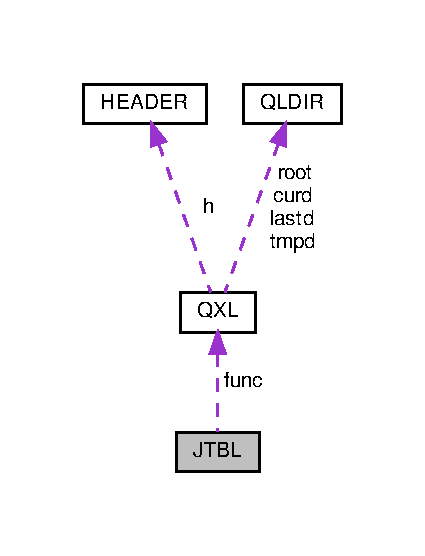
\includegraphics[width=204pt]{struct_j_t_b_l__coll__graph}
\end{center}
\end{figure}
\subsection*{Data Fields}
\begin{DoxyCompactItemize}
\item 
char $\ast$ \hyperlink{struct_j_t_b_l_a5ac083a645d964373f022d03df4849c8}{name}
\item 
\hyperlink{qxltool_8h_a1aef0e7b7f81adb7442c3e9e8fc2d111}{A\+C\+T\+F\+U\+NC} \hyperlink{struct_j_t_b_l_ae6a382beea3f6271f4275fcda5612a65}{func}
\item 
char $\ast$ \hyperlink{struct_j_t_b_l_ac1830353e983a2f22f664cd25d13edf7}{help\+Text}
\item 
short \hyperlink{struct_j_t_b_l_a9872aee74ba489115d3dd6e1f29ca874}{flag}
\end{DoxyCompactItemize}


\subsection{Detailed Description}
Job Table Entry. This structure defines the layout of a single entry in the Q\+X\+Ltool job table. This is used to determine if the commands typed by the user, at the prompt, are valid, and if so, to call the appropriate function to facilitate the command. Parameters are passed in the usual \textquotesingle{}argv\textquotesingle{} manner, much loved in C programs. 

Definition at line 204 of file qxltool.\+h.



\subsection{Field Documentation}
\mbox{\Hypertarget{struct_j_t_b_l_a9872aee74ba489115d3dd6e1f29ca874}\label{struct_j_t_b_l_a9872aee74ba489115d3dd6e1f29ca874}} 
\index{J\+T\+BL@{J\+T\+BL}!flag@{flag}}
\index{flag@{flag}!J\+T\+BL@{J\+T\+BL}}
\subsubsection{\texorpdfstring{flag}{flag}}
{\footnotesize\ttfamily short flag}

T\+O\+DO\+: Purpose to be confirmed! 

Definition at line 209 of file qxltool.\+h.

\mbox{\Hypertarget{struct_j_t_b_l_ae6a382beea3f6271f4275fcda5612a65}\label{struct_j_t_b_l_ae6a382beea3f6271f4275fcda5612a65}} 
\index{J\+T\+BL@{J\+T\+BL}!func@{func}}
\index{func@{func}!J\+T\+BL@{J\+T\+BL}}
\subsubsection{\texorpdfstring{func}{func}}
{\footnotesize\ttfamily \hyperlink{qxltool_8h_a1aef0e7b7f81adb7442c3e9e8fc2d111}{A\+C\+T\+F\+U\+NC} func}

The actual function called. 

Definition at line 207 of file qxltool.\+h.

\mbox{\Hypertarget{struct_j_t_b_l_ac1830353e983a2f22f664cd25d13edf7}\label{struct_j_t_b_l_ac1830353e983a2f22f664cd25d13edf7}} 
\index{J\+T\+BL@{J\+T\+BL}!help\+Text@{help\+Text}}
\index{help\+Text@{help\+Text}!J\+T\+BL@{J\+T\+BL}}
\subsubsection{\texorpdfstring{help\+Text}{helpText}}
{\footnotesize\ttfamily char$\ast$ help\+Text}

Brief help text describing the purpose of this command. 

Definition at line 208 of file qxltool.\+h.

\mbox{\Hypertarget{struct_j_t_b_l_a5ac083a645d964373f022d03df4849c8}\label{struct_j_t_b_l_a5ac083a645d964373f022d03df4849c8}} 
\index{J\+T\+BL@{J\+T\+BL}!name@{name}}
\index{name@{name}!J\+T\+BL@{J\+T\+BL}}
\subsubsection{\texorpdfstring{name}{name}}
{\footnotesize\ttfamily char$\ast$ name}

Command name -\/ as typed by the user at the prompt. 

Definition at line 206 of file qxltool.\+h.



The documentation for this struct was generated from the following file\+:\begin{DoxyCompactItemize}
\item 
/data/\+Source\+Code/qxltools/\hyperlink{qxltool_8h}{qxltool.\+h}\end{DoxyCompactItemize}

\hypertarget{struct_q_l_d_i_r}{}\section{Q\+L\+D\+IR Struct Reference}
\label{struct_q_l_d_i_r}\index{Q\+L\+D\+IR@{Q\+L\+D\+IR}}


{\ttfamily \#include $<$qxltool.\+h$>$}

\subsection*{Data Fields}
\begin{DoxyCompactItemize}
\item 
uint32\+\_\+t \hyperlink{struct_q_l_d_i_r_aebb70c2aab3407a9f05334c47131a43b}{length}
\item 
uint16\+\_\+t \hyperlink{struct_q_l_d_i_r_acb5cfd209ba75c853d03f701e7f91679}{type}
\item 
uint32\+\_\+t \hyperlink{struct_q_l_d_i_r_a1e43bf7d608e87228b625cca2c04d641}{data}
\item 
uint32\+\_\+t \hyperlink{struct_q_l_d_i_r_a11b4492a1b6004ab012f6a7d2525cc3c}{xtra}
\item 
uint16\+\_\+t \hyperlink{struct_q_l_d_i_r_a2b7cf049da1288b6cd8e8380a4455f1e}{nlen}
\item 
uint8\+\_\+t \hyperlink{struct_q_l_d_i_r_a9b899bc186aef90a5f62cf48e1382106}{name} \mbox{[}\hyperlink{qxltool_8h_a723f2285fc63a29eaecf346acf4c184b}{Q\+L\+P\+A\+T\+H\+\_\+\+M\+AX}\mbox{]}
\item 
uint32\+\_\+t \hyperlink{struct_q_l_d_i_r_a52c3c44e31eb489b1913b30e8d1ac88f}{updatedate}
\item 
uint16\+\_\+t \hyperlink{struct_q_l_d_i_r_ab6d7b6f8c2ceaba7acda80aaf05f4899}{version}
\item 
uint16\+\_\+t \hyperlink{struct_q_l_d_i_r_a3a923b731660d8f74929feb1be3bfc56}{map}
\item 
uint32\+\_\+t \hyperlink{struct_q_l_d_i_r_a5ef1b85423e9bee3fd10b60a6f053516}{backupdate}
\end{DoxyCompactItemize}


\subsection{Detailed Description}
\hyperlink{struct_q_x_l}{Q\+XL} Directory Entry. This structure defines the 64 byte (byte aligned) layout of a \hyperlink{struct_q_x_l}{Q\+XL} directory entry. This is a copy of the file header which all files have at the start, although it is never used by the Q\+D\+O\+S/\+S\+M\+SQ system. An empty file, in the directory, is always 64 bytes in size. A zero length file is usually a deleted file, especially if the name length is also zero. 

Definition at line 118 of file qxltool.\+h.



\subsection{Field Documentation}
\mbox{\Hypertarget{struct_q_l_d_i_r_a5ef1b85423e9bee3fd10b60a6f053516}\label{struct_q_l_d_i_r_a5ef1b85423e9bee3fd10b60a6f053516}} 
\index{Q\+L\+D\+IR@{Q\+L\+D\+IR}!backupdate@{backupdate}}
\index{backupdate@{backupdate}!Q\+L\+D\+IR@{Q\+L\+D\+IR}}
\subsubsection{\texorpdfstring{backupdate}{backupdate}}
{\footnotesize\ttfamily uint32\+\_\+t backupdate}

File backup date and time. Used by Win\+Back etc. 

Definition at line 129 of file qxltool.\+h.

\mbox{\Hypertarget{struct_q_l_d_i_r_a1e43bf7d608e87228b625cca2c04d641}\label{struct_q_l_d_i_r_a1e43bf7d608e87228b625cca2c04d641}} 
\index{Q\+L\+D\+IR@{Q\+L\+D\+IR}!data@{data}}
\index{data@{data}!Q\+L\+D\+IR@{Q\+L\+D\+IR}}
\subsubsection{\texorpdfstring{data}{data}}
{\footnotesize\ttfamily uint32\+\_\+t data}

E\+X\+E\+Cutable files\textquotesingle{} require a dataspace for the stack etc. 

Definition at line 122 of file qxltool.\+h.

\mbox{\Hypertarget{struct_q_l_d_i_r_aebb70c2aab3407a9f05334c47131a43b}\label{struct_q_l_d_i_r_aebb70c2aab3407a9f05334c47131a43b}} 
\index{Q\+L\+D\+IR@{Q\+L\+D\+IR}!length@{length}}
\index{length@{length}!Q\+L\+D\+IR@{Q\+L\+D\+IR}}
\subsubsection{\texorpdfstring{length}{length}}
{\footnotesize\ttfamily uint32\+\_\+t length}

File length. Zero is possibly deleted. 64 is an empty file. 

Definition at line 120 of file qxltool.\+h.

\mbox{\Hypertarget{struct_q_l_d_i_r_a3a923b731660d8f74929feb1be3bfc56}\label{struct_q_l_d_i_r_a3a923b731660d8f74929feb1be3bfc56}} 
\index{Q\+L\+D\+IR@{Q\+L\+D\+IR}!map@{map}}
\index{map@{map}!Q\+L\+D\+IR@{Q\+L\+D\+IR}}
\subsubsection{\texorpdfstring{map}{map}}
{\footnotesize\ttfamily uint16\+\_\+t map}

File id number. Index into the map area. 

Definition at line 128 of file qxltool.\+h.

\mbox{\Hypertarget{struct_q_l_d_i_r_a9b899bc186aef90a5f62cf48e1382106}\label{struct_q_l_d_i_r_a9b899bc186aef90a5f62cf48e1382106}} 
\index{Q\+L\+D\+IR@{Q\+L\+D\+IR}!name@{name}}
\index{name@{name}!Q\+L\+D\+IR@{Q\+L\+D\+IR}}
\subsubsection{\texorpdfstring{name}{name}}
{\footnotesize\ttfamily uint8\+\_\+t name\mbox{[}\hyperlink{qxltool_8h_a723f2285fc63a29eaecf346acf4c184b}{Q\+L\+P\+A\+T\+H\+\_\+\+M\+AX}\mbox{]}}

Filename. The full path is here. 36 chracters maximum. 

Definition at line 125 of file qxltool.\+h.

\mbox{\Hypertarget{struct_q_l_d_i_r_a2b7cf049da1288b6cd8e8380a4455f1e}\label{struct_q_l_d_i_r_a2b7cf049da1288b6cd8e8380a4455f1e}} 
\index{Q\+L\+D\+IR@{Q\+L\+D\+IR}!nlen@{nlen}}
\index{nlen@{nlen}!Q\+L\+D\+IR@{Q\+L\+D\+IR}}
\subsubsection{\texorpdfstring{nlen}{nlen}}
{\footnotesize\ttfamily uint16\+\_\+t nlen}

Size of filename. Zero is a deleted file if length is also zero. 

Definition at line 124 of file qxltool.\+h.

\mbox{\Hypertarget{struct_q_l_d_i_r_acb5cfd209ba75c853d03f701e7f91679}\label{struct_q_l_d_i_r_acb5cfd209ba75c853d03f701e7f91679}} 
\index{Q\+L\+D\+IR@{Q\+L\+D\+IR}!type@{type}}
\index{type@{type}!Q\+L\+D\+IR@{Q\+L\+D\+IR}}
\subsubsection{\texorpdfstring{type}{type}}
{\footnotesize\ttfamily uint16\+\_\+t type}

File type\+: 0=Text, Super\+B\+A\+S\+IC source, etc, 1=E\+X\+E\+Cutable, 2=Object (linker input) file, 255=Directory. 

Definition at line 121 of file qxltool.\+h.

\mbox{\Hypertarget{struct_q_l_d_i_r_a52c3c44e31eb489b1913b30e8d1ac88f}\label{struct_q_l_d_i_r_a52c3c44e31eb489b1913b30e8d1ac88f}} 
\index{Q\+L\+D\+IR@{Q\+L\+D\+IR}!updatedate@{updatedate}}
\index{updatedate@{updatedate}!Q\+L\+D\+IR@{Q\+L\+D\+IR}}
\subsubsection{\texorpdfstring{updatedate}{updatedate}}
{\footnotesize\ttfamily uint32\+\_\+t updatedate}

File update date. In the QL epoch (Seconds since 01/01/1970) 

Definition at line 126 of file qxltool.\+h.

\mbox{\Hypertarget{struct_q_l_d_i_r_ab6d7b6f8c2ceaba7acda80aaf05f4899}\label{struct_q_l_d_i_r_ab6d7b6f8c2ceaba7acda80aaf05f4899}} 
\index{Q\+L\+D\+IR@{Q\+L\+D\+IR}!version@{version}}
\index{version@{version}!Q\+L\+D\+IR@{Q\+L\+D\+IR}}
\subsubsection{\texorpdfstring{version}{version}}
{\footnotesize\ttfamily uint16\+\_\+t version}

File version number. 

Definition at line 127 of file qxltool.\+h.

\mbox{\Hypertarget{struct_q_l_d_i_r_a11b4492a1b6004ab012f6a7d2525cc3c}\label{struct_q_l_d_i_r_a11b4492a1b6004ab012f6a7d2525cc3c}} 
\index{Q\+L\+D\+IR@{Q\+L\+D\+IR}!xtra@{xtra}}
\index{xtra@{xtra}!Q\+L\+D\+IR@{Q\+L\+D\+IR}}
\subsubsection{\texorpdfstring{xtra}{xtra}}
{\footnotesize\ttfamily uint32\+\_\+t xtra}

Unused. 

Definition at line 123 of file qxltool.\+h.



The documentation for this struct was generated from the following file\+:\begin{DoxyCompactItemize}
\item 
/data/\+Source\+Code/qxltools/\hyperlink{qxltool_8h}{qxltool.\+h}\end{DoxyCompactItemize}

\hypertarget{struct_q_x_l}{}\section{Q\+XL Struct Reference}
\label{struct_q_x_l}\index{Q\+XL@{Q\+XL}}


{\ttfamily \#include $<$qxltool.\+h$>$}



Collaboration diagram for Q\+XL\+:\nopagebreak
\begin{figure}[H]
\begin{center}
\leavevmode
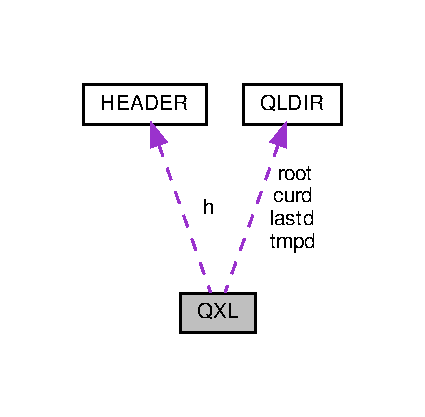
\includegraphics[width=204pt]{struct_q_x_l__coll__graph}
\end{center}
\end{figure}
\subsection*{Data Fields}
\begin{DoxyCompactItemize}
\item 
int \hyperlink{struct_q_x_l_a6f8059414f0228f0256115e024eeed4b}{fd}
\item 
\hyperlink{struct_h_e_a_d_e_r}{H\+E\+A\+D\+ER} \hyperlink{struct_q_x_l_a7599cc5310e4c5370ac2ff59a892244d}{h}
\item 
\hyperlink{struct_q_l_d_i_r}{Q\+L\+D\+IR} \hyperlink{struct_q_x_l_a6de489f08d735198d49d93db47ac17d3}{curd}
\item 
\hyperlink{struct_q_l_d_i_r}{Q\+L\+D\+IR} \hyperlink{struct_q_x_l_a375fb5f40df99977d121396f12103eac}{root}
\item 
\hyperlink{struct_q_l_d_i_r}{Q\+L\+D\+IR} \hyperlink{struct_q_x_l_aa73f3bee736003684c612c765173456b}{tmpd}
\item 
\hyperlink{struct_q_l_d_i_r}{Q\+L\+D\+IR} \hyperlink{struct_q_x_l_ac28f889bad43711b02d0d59d69976ded}{lastd}
\item 
F\+I\+LE $\ast$ \hyperlink{struct_q_x_l_aa065f30aa9f5f9a42132c82c787ee70b}{fp}
\item 
short \hyperlink{struct_q_x_l_ab6947e12da3463e7a671017f8804ebc8}{close}
\item 
char \hyperlink{struct_q_x_l_a7b855d6690caa0e60d0320cafd38051d}{fn} \mbox{[}P\+A\+T\+H\+\_\+\+M\+AX\mbox{]}
\item 
int \hyperlink{struct_q_x_l_a1ea5d0cb93f22f7d0fdf804bd68c3326}{mode}
\item 
short \hyperlink{struct_q_x_l_a1e2da7ce56bf4f62a21da3ea15b88805}{fmode}
\end{DoxyCompactItemize}


\subsection{Detailed Description}
\hyperlink{struct_q_x_l}{Q\+XL} Structure. This structure is used internally by Q\+X\+L\+Tool, to pass around details of the \hyperlink{struct_q_x_l}{Q\+XL} file being processed. 

Definition at line 154 of file qxltool.\+h.



\subsection{Field Documentation}
\mbox{\Hypertarget{struct_q_x_l_ab6947e12da3463e7a671017f8804ebc8}\label{struct_q_x_l_ab6947e12da3463e7a671017f8804ebc8}} 
\index{Q\+XL@{Q\+XL}!close@{close}}
\index{close@{close}!Q\+XL@{Q\+XL}}
\subsubsection{\texorpdfstring{close}{close}}
{\footnotesize\ttfamily short close}

T\+O\+DO\+: To be confirmed. 

Definition at line 163 of file qxltool.\+h.

\mbox{\Hypertarget{struct_q_x_l_a6de489f08d735198d49d93db47ac17d3}\label{struct_q_x_l_a6de489f08d735198d49d93db47ac17d3}} 
\index{Q\+XL@{Q\+XL}!curd@{curd}}
\index{curd@{curd}!Q\+XL@{Q\+XL}}
\subsubsection{\texorpdfstring{curd}{curd}}
{\footnotesize\ttfamily \hyperlink{struct_q_l_d_i_r}{Q\+L\+D\+IR} curd}

Directory entry for the current directory. 

Definition at line 158 of file qxltool.\+h.

\mbox{\Hypertarget{struct_q_x_l_a6f8059414f0228f0256115e024eeed4b}\label{struct_q_x_l_a6f8059414f0228f0256115e024eeed4b}} 
\index{Q\+XL@{Q\+XL}!fd@{fd}}
\index{fd@{fd}!Q\+XL@{Q\+XL}}
\subsubsection{\texorpdfstring{fd}{fd}}
{\footnotesize\ttfamily int fd}

File descriptor to access the underlying \hyperlink{struct_q_x_l}{Q\+XL} file. 

Definition at line 156 of file qxltool.\+h.

\mbox{\Hypertarget{struct_q_x_l_a1e2da7ce56bf4f62a21da3ea15b88805}\label{struct_q_x_l_a1e2da7ce56bf4f62a21da3ea15b88805}} 
\index{Q\+XL@{Q\+XL}!fmode@{fmode}}
\index{fmode@{fmode}!Q\+XL@{Q\+XL}}
\subsubsection{\texorpdfstring{fmode}{fmode}}
{\footnotesize\ttfamily short fmode}

T\+O\+DO\+: To be confirmed. 

Definition at line 166 of file qxltool.\+h.

\mbox{\Hypertarget{struct_q_x_l_a7b855d6690caa0e60d0320cafd38051d}\label{struct_q_x_l_a7b855d6690caa0e60d0320cafd38051d}} 
\index{Q\+XL@{Q\+XL}!fn@{fn}}
\index{fn@{fn}!Q\+XL@{Q\+XL}}
\subsubsection{\texorpdfstring{fn}{fn}}
{\footnotesize\ttfamily char fn\mbox{[}P\+A\+T\+H\+\_\+\+M\+AX\mbox{]}}

Underlying \hyperlink{struct_q_x_l}{Q\+XL} filename on the OS. 

Definition at line 164 of file qxltool.\+h.

\mbox{\Hypertarget{struct_q_x_l_aa065f30aa9f5f9a42132c82c787ee70b}\label{struct_q_x_l_aa065f30aa9f5f9a42132c82c787ee70b}} 
\index{Q\+XL@{Q\+XL}!fp@{fp}}
\index{fp@{fp}!Q\+XL@{Q\+XL}}
\subsubsection{\texorpdfstring{fp}{fp}}
{\footnotesize\ttfamily F\+I\+LE$\ast$ fp}

T\+O\+DO\+: To be confirmed. 

Definition at line 162 of file qxltool.\+h.

\mbox{\Hypertarget{struct_q_x_l_a7599cc5310e4c5370ac2ff59a892244d}\label{struct_q_x_l_a7599cc5310e4c5370ac2ff59a892244d}} 
\index{Q\+XL@{Q\+XL}!h@{h}}
\index{h@{h}!Q\+XL@{Q\+XL}}
\subsubsection{\texorpdfstring{h}{h}}
{\footnotesize\ttfamily \hyperlink{struct_h_e_a_d_e_r}{H\+E\+A\+D\+ER} h}

\hyperlink{struct_q_x_l}{Q\+XL} file\textquotesingle{}s header. 

Definition at line 157 of file qxltool.\+h.

\mbox{\Hypertarget{struct_q_x_l_ac28f889bad43711b02d0d59d69976ded}\label{struct_q_x_l_ac28f889bad43711b02d0d59d69976ded}} 
\index{Q\+XL@{Q\+XL}!lastd@{lastd}}
\index{lastd@{lastd}!Q\+XL@{Q\+XL}}
\subsubsection{\texorpdfstring{lastd}{lastd}}
{\footnotesize\ttfamily \hyperlink{struct_q_l_d_i_r}{Q\+L\+D\+IR} lastd}

T\+O\+DO\+: To be confirmed. 

Definition at line 161 of file qxltool.\+h.

\mbox{\Hypertarget{struct_q_x_l_a1ea5d0cb93f22f7d0fdf804bd68c3326}\label{struct_q_x_l_a1ea5d0cb93f22f7d0fdf804bd68c3326}} 
\index{Q\+XL@{Q\+XL}!mode@{mode}}
\index{mode@{mode}!Q\+XL@{Q\+XL}}
\subsubsection{\texorpdfstring{mode}{mode}}
{\footnotesize\ttfamily int mode}

T\+O\+DO\+: To be confirmed. 

Definition at line 165 of file qxltool.\+h.

\mbox{\Hypertarget{struct_q_x_l_a375fb5f40df99977d121396f12103eac}\label{struct_q_x_l_a375fb5f40df99977d121396f12103eac}} 
\index{Q\+XL@{Q\+XL}!root@{root}}
\index{root@{root}!Q\+XL@{Q\+XL}}
\subsubsection{\texorpdfstring{root}{root}}
{\footnotesize\ttfamily \hyperlink{struct_q_l_d_i_r}{Q\+L\+D\+IR} root}

Directory entry for the root directory. 

Definition at line 159 of file qxltool.\+h.

\mbox{\Hypertarget{struct_q_x_l_aa73f3bee736003684c612c765173456b}\label{struct_q_x_l_aa73f3bee736003684c612c765173456b}} 
\index{Q\+XL@{Q\+XL}!tmpd@{tmpd}}
\index{tmpd@{tmpd}!Q\+XL@{Q\+XL}}
\subsubsection{\texorpdfstring{tmpd}{tmpd}}
{\footnotesize\ttfamily \hyperlink{struct_q_l_d_i_r}{Q\+L\+D\+IR} tmpd}

T\+O\+DO\+: To be confirmed. 

Definition at line 160 of file qxltool.\+h.



The documentation for this struct was generated from the following file\+:\begin{DoxyCompactItemize}
\item 
/data/\+Source\+Code/qxltools/\hyperlink{qxltool_8h}{qxltool.\+h}\end{DoxyCompactItemize}

\hypertarget{struct_x_t_c_c}{}\section{X\+T\+CC Struct Reference}
\label{struct_x_t_c_c}\index{X\+T\+CC@{X\+T\+CC}}


{\ttfamily \#include $<$qxltool.\+h$>$}

\subsection*{Data Fields}
\begin{DoxyCompactItemize}
\item 
\begin{tabbing}
xx\=xx\=xx\=xx\=xx\=xx\=xx\=xx\=xx\=\kill
union \{\\
\>char \hyperlink{struct_x_t_c_c_acd9081c4e246dfc8ecf272a9ccb10624}{xtcc} \mbox{[}4\mbox{]}\\
\>long \hyperlink{struct_x_t_c_c_a3162ada50d1df39e0f0555ea3d60dea1}{x}\\
\} \hyperlink{struct_x_t_c_c_ac3cd33d0da064be57dbfdfe529905ff2}{x}\\

\end{tabbing}\item 
uint32\+\_\+t \hyperlink{struct_x_t_c_c_a980b74c86756f84742ba39d62d733e25}{dlen}
\end{DoxyCompactItemize}


\subsection{Detailed Description}
\hyperlink{struct_x_t_c_c}{X\+T\+CC} Data block. This is an 8 byte block, added to the end of a file created on a non-\/\+Q\+D\+O\+S/\+S\+M\+SQ system, which records the dataspace requirements for executable files. This, with the correct software on Q\+D\+O\+S/\+S\+M\+SQ, allows for the transfer of files between operating systems, without loss of the header data. 

Definition at line 137 of file qxltool.\+h.



\subsection{Field Documentation}
\mbox{\Hypertarget{struct_x_t_c_c_a980b74c86756f84742ba39d62d733e25}\label{struct_x_t_c_c_a980b74c86756f84742ba39d62d733e25}} 
\index{X\+T\+CC@{X\+T\+CC}!dlen@{dlen}}
\index{dlen@{dlen}!X\+T\+CC@{X\+T\+CC}}
\subsubsection{\texorpdfstring{dlen}{dlen}}
{\footnotesize\ttfamily uint32\+\_\+t dlen}

Dataspace required when running on Q\+D\+O\+S/\+S\+M\+SQ. 

Definition at line 144 of file qxltool.\+h.

\mbox{\Hypertarget{struct_x_t_c_c_a3162ada50d1df39e0f0555ea3d60dea1}\label{struct_x_t_c_c_a3162ada50d1df39e0f0555ea3d60dea1}} 
\index{X\+T\+CC@{X\+T\+CC}!x@{x}}
\index{x@{x}!X\+T\+CC@{X\+T\+CC}}
\subsubsection{\texorpdfstring{x}{x}\hspace{0.1cm}{\footnotesize\ttfamily [1/2]}}
{\footnotesize\ttfamily long x}

T\+O\+DO\+: Purpose to be confirmed. 

Definition at line 142 of file qxltool.\+h.

\mbox{\Hypertarget{struct_x_t_c_c_ac3cd33d0da064be57dbfdfe529905ff2}\label{struct_x_t_c_c_ac3cd33d0da064be57dbfdfe529905ff2}} 
\index{X\+T\+CC@{X\+T\+CC}!x@{x}}
\index{x@{x}!X\+T\+CC@{X\+T\+CC}}
\subsubsection{\texorpdfstring{x}{x}\hspace{0.1cm}{\footnotesize\ttfamily [2/2]}}
{\footnotesize\ttfamily union \{ ... \}   x}

\mbox{\Hypertarget{struct_x_t_c_c_acd9081c4e246dfc8ecf272a9ccb10624}\label{struct_x_t_c_c_acd9081c4e246dfc8ecf272a9ccb10624}} 
\index{X\+T\+CC@{X\+T\+CC}!xtcc@{xtcc}}
\index{xtcc@{xtcc}!X\+T\+CC@{X\+T\+CC}}
\subsubsection{\texorpdfstring{xtcc}{xtcc}}
{\footnotesize\ttfamily char xtcc\mbox{[}4\mbox{]}}

Marker flag. \textquotesingle{}X\+Tcc\textquotesingle{}. 

Definition at line 141 of file qxltool.\+h.



The documentation for this struct was generated from the following file\+:\begin{DoxyCompactItemize}
\item 
/data/\+Source\+Code/qxltools/\hyperlink{qxltool_8h}{qxltool.\+h}\end{DoxyCompactItemize}

\chapter{File Documentation}
\hypertarget{confdefs_8h}{}\section{/data/\+Source\+Code/qxltools/confdefs.h File Reference}
\label{confdefs_8h}\index{/data/\+Source\+Code/qxltools/confdefs.\+h@{/data/\+Source\+Code/qxltools/confdefs.\+h}}

\hypertarget{qxltool_8c}{}\section{/data/\+Source\+Code/qxltools/qxltool.c File Reference}
\label{qxltool_8c}\index{/data/\+Source\+Code/qxltools/qxltool.\+c@{/data/\+Source\+Code/qxltools/qxltool.\+c}}
{\ttfamily \#include $<$stdio.\+h$>$}\newline
{\ttfamily \#include $<$stdlib.\+h$>$}\newline
{\ttfamily \#include $<$fcntl.\+h$>$}\newline
{\ttfamily \#include $<$string.\+h$>$}\newline
{\ttfamily \#include $<$ctype.\+h$>$}\newline
{\ttfamily \#include $<$limits.\+h$>$}\newline
{\ttfamily \#include $<$signal.\+h$>$}\newline
{\ttfamily \#include $<$sys/stat.\+h$>$}\newline
{\ttfamily \#include $<$stddef.\+h$>$}\newline
{\ttfamily \#include $<$sys/types.\+h$>$}\newline
{\ttfamily \#include $<$math.\+h$>$}\newline
{\ttfamily \#include \char`\"{}qxltool.\+h\char`\"{}}\newline
Include dependency graph for qxltool.\+c\+:\nopagebreak
\begin{figure}[H]
\begin{center}
\leavevmode
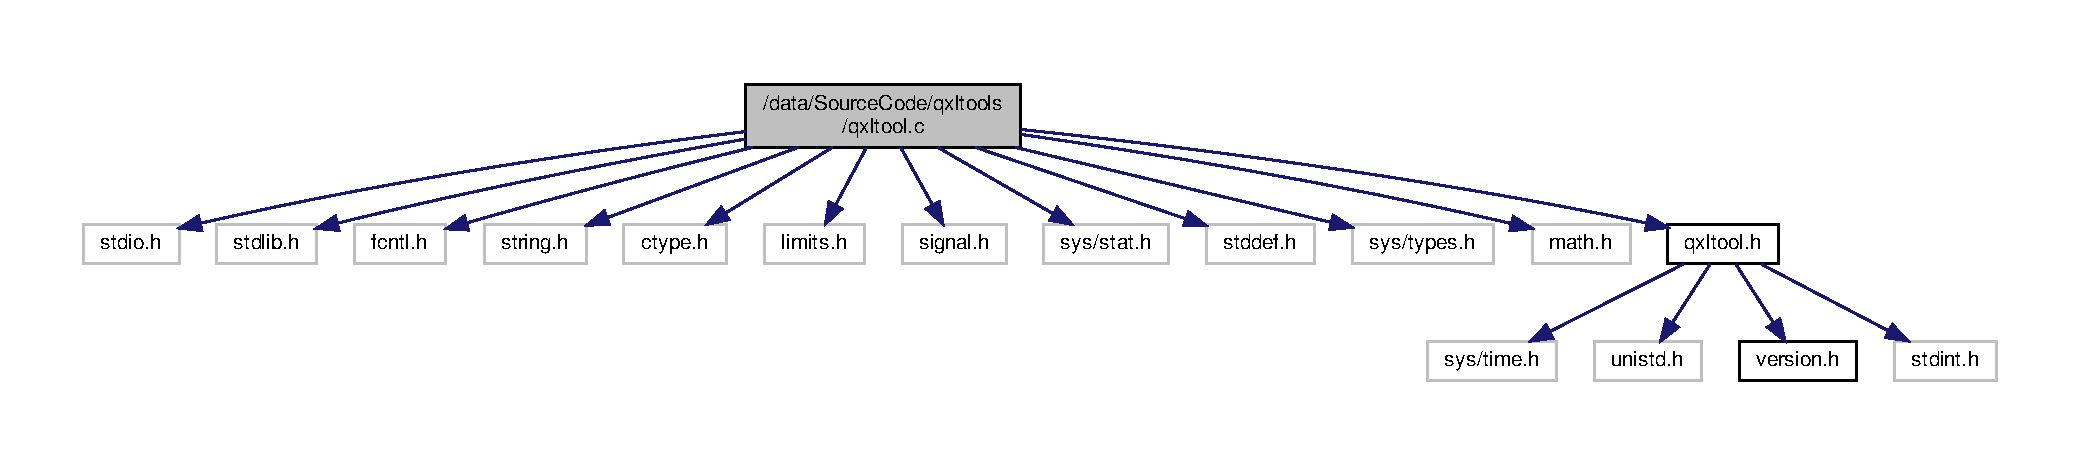
\includegraphics[width=350pt]{qxltool_8c__incl}
\end{center}
\end{figure}
\subsection*{Macros}
\begin{DoxyCompactItemize}
\item 
\#define \hyperlink{qxltool_8c_a369266c24eacffb87046522897a570d5}{\+\_\+\+G\+N\+U\+\_\+\+S\+O\+U\+R\+CE}
\item 
\#define \hyperlink{qxltool_8c_aba5465c8b8b7553619d28567aa3b0bc1}{L\+I\+N\+S\+IZ}~(256)
\item 
\#define \hyperlink{qxltool_8c_a0d930c36f0cf839b5ffc26ebc4ac3779}{SW}(a,  c)~(a)-\/$>$c = \hyperlink{qxltool_8c_a0cd373ef29b0b7e44d45e135670461f1}{swapword}((a)-\/$>$c)
\item 
\#define \hyperlink{qxltool_8c_a7c551f029751a593bb01823e9b73cb52}{SL}(a,  c)~(a)-\/$>$c = \hyperlink{qxltool_8c_a36510986cf07803481e211eb18e66fed}{swaplong}((a)-\/$>$c)
\item 
\#define \hyperlink{qxltool_8c_ad41e3158a654dd4dfdab19d97745698a}{F\+N\+M\+\_\+\+C\+A\+S\+E\+F\+O\+LD}~0
\item 
\#define \hyperlink{qxltool_8c_a36c8e82ccce7b6236f41bd956a8b4159}{D\+U\+P\+C\+MD}(b)~strdup(b)
\item 
\#define \hyperlink{qxltool_8c_a2358e43204758a45d3054f334bfb0ab0}{C\+O\+P\+Y\+\_\+\+IN}~\textquotesingle{}I\textquotesingle{}
\item 
\#define \hyperlink{qxltool_8c_a1bdbfd56ff8ac71aef45ea35857f7213}{C\+O\+P\+Y\+\_\+\+O\+UT}~\textquotesingle{}O\textquotesingle{}
\item 
\#define \hyperlink{qxltool_8c_a95cf1ca63ff303311d342d1a53d51f38}{S\+EP}~\textquotesingle{}\+:\textquotesingle{}
\end{DoxyCompactItemize}
\subsection*{Functions}
\begin{DoxyCompactItemize}
\item 
char $\ast$ \hyperlink{qxltool_8c_a20c04ba230adfdea1a6db4f5f12e5447}{stpcpy} (char $\ast$s1, char $\ast$s2)
\item 
u\+\_\+short \hyperlink{qxltool_8c_a0cd373ef29b0b7e44d45e135670461f1}{swapword} (u\+\_\+short val)
\item 
u\+\_\+long \hyperlink{qxltool_8c_a36510986cf07803481e211eb18e66fed}{swaplong} (u\+\_\+long val)
\item 
char $\ast$ \hyperlink{qxltool_8c_a4bede698ddab5756c143e5c1b874b0dd}{R\+E\+A\+D\+L\+I\+NE} (char $\ast$a, char $\ast$b)
\item 
void \hyperlink{qxltool_8c_aed4a6358dffdf7637bf19261de8774f9}{F\+R\+E\+E\+C\+MD} (char $\ast$a, char $\ast$b)
\item 
int \hyperlink{qxltool_8c_a0c99d968a34e803d378692bde2e3f18f}{main} (int ac, char $\ast$$\ast$av)
\end{DoxyCompactItemize}


\subsection{Macro Definition Documentation}
\mbox{\Hypertarget{qxltool_8c_a369266c24eacffb87046522897a570d5}\label{qxltool_8c_a369266c24eacffb87046522897a570d5}} 
\index{qxltool.\+c@{qxltool.\+c}!\+\_\+\+G\+N\+U\+\_\+\+S\+O\+U\+R\+CE@{\+\_\+\+G\+N\+U\+\_\+\+S\+O\+U\+R\+CE}}
\index{\+\_\+\+G\+N\+U\+\_\+\+S\+O\+U\+R\+CE@{\+\_\+\+G\+N\+U\+\_\+\+S\+O\+U\+R\+CE}!qxltool.\+c@{qxltool.\+c}}
\subsubsection{\texorpdfstring{\+\_\+\+G\+N\+U\+\_\+\+S\+O\+U\+R\+CE}{\_GNU\_SOURCE}}
{\footnotesize\ttfamily \#define \+\_\+\+G\+N\+U\+\_\+\+S\+O\+U\+R\+CE}



Definition at line 11 of file qxltool.\+c.

\mbox{\Hypertarget{qxltool_8c_a2358e43204758a45d3054f334bfb0ab0}\label{qxltool_8c_a2358e43204758a45d3054f334bfb0ab0}} 
\index{qxltool.\+c@{qxltool.\+c}!C\+O\+P\+Y\+\_\+\+IN@{C\+O\+P\+Y\+\_\+\+IN}}
\index{C\+O\+P\+Y\+\_\+\+IN@{C\+O\+P\+Y\+\_\+\+IN}!qxltool.\+c@{qxltool.\+c}}
\subsubsection{\texorpdfstring{C\+O\+P\+Y\+\_\+\+IN}{COPY\_IN}}
{\footnotesize\ttfamily \#define C\+O\+P\+Y\+\_\+\+IN~\textquotesingle{}I\textquotesingle{}}



Definition at line 2319 of file qxltool.\+c.

\mbox{\Hypertarget{qxltool_8c_a1bdbfd56ff8ac71aef45ea35857f7213}\label{qxltool_8c_a1bdbfd56ff8ac71aef45ea35857f7213}} 
\index{qxltool.\+c@{qxltool.\+c}!C\+O\+P\+Y\+\_\+\+O\+UT@{C\+O\+P\+Y\+\_\+\+O\+UT}}
\index{C\+O\+P\+Y\+\_\+\+O\+UT@{C\+O\+P\+Y\+\_\+\+O\+UT}!qxltool.\+c@{qxltool.\+c}}
\subsubsection{\texorpdfstring{C\+O\+P\+Y\+\_\+\+O\+UT}{COPY\_OUT}}
{\footnotesize\ttfamily \#define C\+O\+P\+Y\+\_\+\+O\+UT~\textquotesingle{}O\textquotesingle{}}



Definition at line 2320 of file qxltool.\+c.

\mbox{\Hypertarget{qxltool_8c_a36c8e82ccce7b6236f41bd956a8b4159}\label{qxltool_8c_a36c8e82ccce7b6236f41bd956a8b4159}} 
\index{qxltool.\+c@{qxltool.\+c}!D\+U\+P\+C\+MD@{D\+U\+P\+C\+MD}}
\index{D\+U\+P\+C\+MD@{D\+U\+P\+C\+MD}!qxltool.\+c@{qxltool.\+c}}
\subsubsection{\texorpdfstring{D\+U\+P\+C\+MD}{DUPCMD}}
{\footnotesize\ttfamily \#define D\+U\+P\+C\+MD(\begin{DoxyParamCaption}\item[{}]{b }\end{DoxyParamCaption})~strdup(b)}



Definition at line 2054 of file qxltool.\+c.

\mbox{\Hypertarget{qxltool_8c_ad41e3158a654dd4dfdab19d97745698a}\label{qxltool_8c_ad41e3158a654dd4dfdab19d97745698a}} 
\index{qxltool.\+c@{qxltool.\+c}!F\+N\+M\+\_\+\+C\+A\+S\+E\+F\+O\+LD@{F\+N\+M\+\_\+\+C\+A\+S\+E\+F\+O\+LD}}
\index{F\+N\+M\+\_\+\+C\+A\+S\+E\+F\+O\+LD@{F\+N\+M\+\_\+\+C\+A\+S\+E\+F\+O\+LD}!qxltool.\+c@{qxltool.\+c}}
\subsubsection{\texorpdfstring{F\+N\+M\+\_\+\+C\+A\+S\+E\+F\+O\+LD}{FNM\_CASEFOLD}}
{\footnotesize\ttfamily \#define F\+N\+M\+\_\+\+C\+A\+S\+E\+F\+O\+LD~0}



Definition at line 385 of file qxltool.\+c.

\mbox{\Hypertarget{qxltool_8c_aba5465c8b8b7553619d28567aa3b0bc1}\label{qxltool_8c_aba5465c8b8b7553619d28567aa3b0bc1}} 
\index{qxltool.\+c@{qxltool.\+c}!L\+I\+N\+S\+IZ@{L\+I\+N\+S\+IZ}}
\index{L\+I\+N\+S\+IZ@{L\+I\+N\+S\+IZ}!qxltool.\+c@{qxltool.\+c}}
\subsubsection{\texorpdfstring{L\+I\+N\+S\+IZ}{LINSIZ}}
{\footnotesize\ttfamily \#define L\+I\+N\+S\+IZ~(256)}



Definition at line 59 of file qxltool.\+c.

\mbox{\Hypertarget{qxltool_8c_a95cf1ca63ff303311d342d1a53d51f38}\label{qxltool_8c_a95cf1ca63ff303311d342d1a53d51f38}} 
\index{qxltool.\+c@{qxltool.\+c}!S\+EP@{S\+EP}}
\index{S\+EP@{S\+EP}!qxltool.\+c@{qxltool.\+c}}
\subsubsection{\texorpdfstring{S\+EP}{SEP}}
{\footnotesize\ttfamily \#define S\+EP~\textquotesingle{}\+:\textquotesingle{}}



Definition at line 2325 of file qxltool.\+c.

\mbox{\Hypertarget{qxltool_8c_a7c551f029751a593bb01823e9b73cb52}\label{qxltool_8c_a7c551f029751a593bb01823e9b73cb52}} 
\index{qxltool.\+c@{qxltool.\+c}!SL@{SL}}
\index{SL@{SL}!qxltool.\+c@{qxltool.\+c}}
\subsubsection{\texorpdfstring{SL}{SL}}
{\footnotesize\ttfamily \#define SL(\begin{DoxyParamCaption}\item[{}]{a,  }\item[{}]{c }\end{DoxyParamCaption})~(a)-\/$>$c = \hyperlink{qxltool_8c_a36510986cf07803481e211eb18e66fed}{swaplong}((a)-\/$>$c)}



Definition at line 99 of file qxltool.\+c.

\mbox{\Hypertarget{qxltool_8c_a0d930c36f0cf839b5ffc26ebc4ac3779}\label{qxltool_8c_a0d930c36f0cf839b5ffc26ebc4ac3779}} 
\index{qxltool.\+c@{qxltool.\+c}!SW@{SW}}
\index{SW@{SW}!qxltool.\+c@{qxltool.\+c}}
\subsubsection{\texorpdfstring{SW}{SW}}
{\footnotesize\ttfamily \#define SW(\begin{DoxyParamCaption}\item[{}]{a,  }\item[{}]{c }\end{DoxyParamCaption})~(a)-\/$>$c = \hyperlink{qxltool_8c_a0cd373ef29b0b7e44d45e135670461f1}{swapword}((a)-\/$>$c)}



Definition at line 98 of file qxltool.\+c.



\subsection{Function Documentation}
\mbox{\Hypertarget{qxltool_8c_aed4a6358dffdf7637bf19261de8774f9}\label{qxltool_8c_aed4a6358dffdf7637bf19261de8774f9}} 
\index{qxltool.\+c@{qxltool.\+c}!F\+R\+E\+E\+C\+MD@{F\+R\+E\+E\+C\+MD}}
\index{F\+R\+E\+E\+C\+MD@{F\+R\+E\+E\+C\+MD}!qxltool.\+c@{qxltool.\+c}}
\subsubsection{\texorpdfstring{F\+R\+E\+E\+C\+M\+D()}{FREECMD()}}
{\footnotesize\ttfamily void F\+R\+E\+E\+C\+MD (\begin{DoxyParamCaption}\item[{char $\ast$}]{a,  }\item[{char $\ast$}]{b }\end{DoxyParamCaption})}



Definition at line 2046 of file qxltool.\+c.

\mbox{\Hypertarget{qxltool_8c_a0c99d968a34e803d378692bde2e3f18f}\label{qxltool_8c_a0c99d968a34e803d378692bde2e3f18f}} 
\index{qxltool.\+c@{qxltool.\+c}!main@{main}}
\index{main@{main}!qxltool.\+c@{qxltool.\+c}}
\subsubsection{\texorpdfstring{main()}{main()}}
{\footnotesize\ttfamily int main (\begin{DoxyParamCaption}\item[{int}]{ac,  }\item[{char $\ast$$\ast$}]{av }\end{DoxyParamCaption})}



Definition at line 2615 of file qxltool.\+c.

\mbox{\Hypertarget{qxltool_8c_a4bede698ddab5756c143e5c1b874b0dd}\label{qxltool_8c_a4bede698ddab5756c143e5c1b874b0dd}} 
\index{qxltool.\+c@{qxltool.\+c}!R\+E\+A\+D\+L\+I\+NE@{R\+E\+A\+D\+L\+I\+NE}}
\index{R\+E\+A\+D\+L\+I\+NE@{R\+E\+A\+D\+L\+I\+NE}!qxltool.\+c@{qxltool.\+c}}
\subsubsection{\texorpdfstring{R\+E\+A\+D\+L\+I\+N\+E()}{READLINE()}}
{\footnotesize\ttfamily char$\ast$ R\+E\+A\+D\+L\+I\+NE (\begin{DoxyParamCaption}\item[{char $\ast$}]{a,  }\item[{char $\ast$}]{b }\end{DoxyParamCaption})}



Definition at line 2024 of file qxltool.\+c.

\mbox{\Hypertarget{qxltool_8c_a20c04ba230adfdea1a6db4f5f12e5447}\label{qxltool_8c_a20c04ba230adfdea1a6db4f5f12e5447}} 
\index{qxltool.\+c@{qxltool.\+c}!stpcpy@{stpcpy}}
\index{stpcpy@{stpcpy}!qxltool.\+c@{qxltool.\+c}}
\subsubsection{\texorpdfstring{stpcpy()}{stpcpy()}}
{\footnotesize\ttfamily char$\ast$ stpcpy (\begin{DoxyParamCaption}\item[{char $\ast$}]{s1,  }\item[{char $\ast$}]{s2 }\end{DoxyParamCaption})}



Definition at line 70 of file qxltool.\+c.

\mbox{\Hypertarget{qxltool_8c_a36510986cf07803481e211eb18e66fed}\label{qxltool_8c_a36510986cf07803481e211eb18e66fed}} 
\index{qxltool.\+c@{qxltool.\+c}!swaplong@{swaplong}}
\index{swaplong@{swaplong}!qxltool.\+c@{qxltool.\+c}}
\subsubsection{\texorpdfstring{swaplong()}{swaplong()}}
{\footnotesize\ttfamily u\+\_\+long swaplong (\begin{DoxyParamCaption}\item[{u\+\_\+long}]{val }\end{DoxyParamCaption})\hspace{0.3cm}{\ttfamily [inline]}}



Definition at line 92 of file qxltool.\+c.

Here is the call graph for this function\+:\nopagebreak
\begin{figure}[H]
\begin{center}
\leavevmode
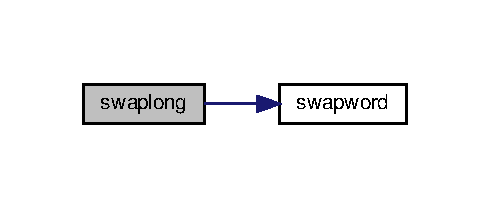
\includegraphics[width=235pt]{qxltool_8c_a36510986cf07803481e211eb18e66fed_cgraph}
\end{center}
\end{figure}
\mbox{\Hypertarget{qxltool_8c_a0cd373ef29b0b7e44d45e135670461f1}\label{qxltool_8c_a0cd373ef29b0b7e44d45e135670461f1}} 
\index{qxltool.\+c@{qxltool.\+c}!swapword@{swapword}}
\index{swapword@{swapword}!qxltool.\+c@{qxltool.\+c}}
\subsubsection{\texorpdfstring{swapword()}{swapword()}}
{\footnotesize\ttfamily u\+\_\+short swapword (\begin{DoxyParamCaption}\item[{u\+\_\+short}]{val }\end{DoxyParamCaption})\hspace{0.3cm}{\ttfamily [inline]}}



Definition at line 83 of file qxltool.\+c.

Here is the caller graph for this function\+:\nopagebreak
\begin{figure}[H]
\begin{center}
\leavevmode
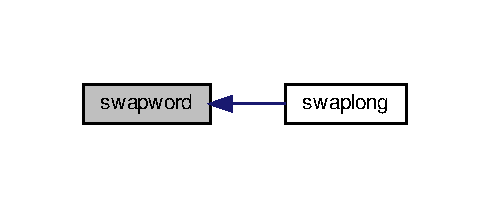
\includegraphics[width=235pt]{qxltool_8c_a0cd373ef29b0b7e44d45e135670461f1_icgraph}
\end{center}
\end{figure}

\hypertarget{qxltool_8h}{}\section{/data/\+Source\+Code/qxltools/qxltool.h File Reference}
\label{qxltool_8h}\index{/data/\+Source\+Code/qxltools/qxltool.\+h@{/data/\+Source\+Code/qxltools/qxltool.\+h}}
{\ttfamily \#include $<$sys/time.\+h$>$}\newline
{\ttfamily \#include $<$unistd.\+h$>$}\newline
{\ttfamily \#include \char`\"{}version.\+h\char`\"{}}\newline
{\ttfamily \#include $<$stdint.\+h$>$}\newline
Include dependency graph for qxltool.\+h\+:\nopagebreak
\begin{figure}[H]
\begin{center}
\leavevmode
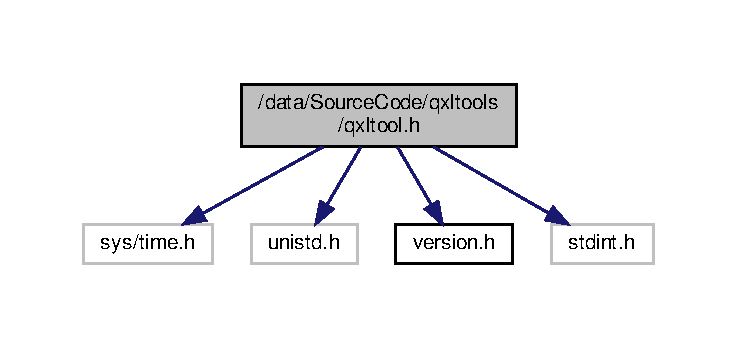
\includegraphics[width=350pt]{qxltool_8h__incl}
\end{center}
\end{figure}
This graph shows which files directly or indirectly include this file\+:\nopagebreak
\begin{figure}[H]
\begin{center}
\leavevmode
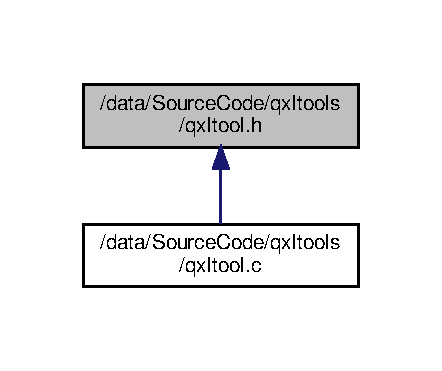
\includegraphics[width=212pt]{qxltool_8h__dep__incl}
\end{center}
\end{figure}
\subsection*{Data Structures}
\begin{DoxyCompactItemize}
\item 
struct \hyperlink{struct_h_e_a_d_e_r}{H\+E\+A\+D\+ER}
\item 
struct \hyperlink{struct_q_l_d_i_r}{Q\+L\+D\+IR}
\item 
struct \hyperlink{struct_x_t_c_c}{X\+T\+CC}
\item 
struct \hyperlink{struct_q_x_l}{Q\+XL}
\item 
struct \hyperlink{struct_j_t_b_l}{J\+T\+BL}
\end{DoxyCompactItemize}
\subsection*{Macros}
\begin{DoxyCompactItemize}
\item 
\#define \hyperlink{qxltool_8h_ae1fa6471aea312a8194a3c14b698a7b9}{U\+N\+I\+X2\+QL}~283996800
\item 
\#define \hyperlink{qxltool_8h_a9a9ce2ac0916cc9d64baf778a1121283}{Q\+L2\+U\+N\+IX}~-\/(\hyperlink{qxltool_8h_ae1fa6471aea312a8194a3c14b698a7b9}{U\+N\+I\+X2\+QL})
\item 
\#define \hyperlink{qxltool_8h_ab31dd96cbaf5918f850bc5e2df176eef}{V\+E\+R\+S\+TR}~\hyperlink{version_8h_a1c6d5de492ac61ad29aec7aa9a436bbf}{V\+E\+R\+S\+I\+ON} \char`\"{}, \char`\"{} \+\_\+\+\_\+\+D\+A\+T\+E\+\_\+\+\_\+
\item 
\#define \hyperlink{qxltool_8h_a36d525cf4d116b2fe4ecc00222b256f1}{P\+A\+C\+K\+ED}
\item 
\#define \hyperlink{qxltool_8h_aebaa75918caa819e6ca7fd17e839ff99}{D\+E\+F\+Q\+XL}~\char`\"{}win2\+\_\+tmp\+\_\+qxl.\+win\char`\"{}
\item 
\#define \hyperlink{qxltool_8h_a9fec70a17d0bcef23cf03c45a7b7caba}{T\+A\+R\+G\+ET}~\char`\"{}Q\+D\+OS\char`\"{}
\item 
\#define \hyperlink{qxltool_8h_a0db8a9b5ad5a66e4adc36d0ba68735c8}{S\+H\+E\+LL}~\char`\"{}S\+H\+E\+LL\char`\"{}
\item 
\#define \hyperlink{qxltool_8h_a723f2285fc63a29eaecf346acf4c184b}{Q\+L\+P\+A\+T\+H\+\_\+\+M\+AX}~36
\item 
\#define \hyperlink{qxltool_8h_a36fa9b2e726512bc17a7a6d3e39002be}{O\+\_\+\+B\+I\+N\+A\+RY}~0
\item 
\#define \hyperlink{qxltool_8h_ae7b5e4a4f47370e09fe006aa77a70b5e}{offsetof}(sname,  fname)~((long)\&((sname $\ast$)0)-\/$>$fname)
\item 
\#define \hyperlink{qxltool_8h_a8230adff64fe581cfdf04be6d8e91bcd}{S\+E\+C\+T\+O\+R\+S\+I\+ZE}~512
\item 
\#define \hyperlink{qxltool_8h_aa3f3bd1e526bb7836483dfeff1cd54b9}{D\+O\+\_\+\+R\+E\+C\+U\+R\+SE}~(1 $<$$<$ 0)
\item 
\#define \hyperlink{qxltool_8h_a956fd3a775245775c41f035fd364ea73}{D\+O\+\_\+\+B\+E\+ST}~(1 $<$$<$ 1)
\item 
\#define \hyperlink{qxltool_8h_a4261e7f0e09774710c533a9ebee35986}{D\+O\+\_\+\+W\+I\+LD}~(1 $<$$<$ 2)
\item 
\#define \hyperlink{qxltool_8h_a9b86083c851e711fb0fe852fe37cd858}{Q\+X\+\_\+\+T\+E\+XT}~(1 $<$$<$ 0)
\item 
\#define \hyperlink{qxltool_8h_ae8c0ec9696a03336d1e19cfc2e98e3af}{Q\+X\+\_\+\+O\+P\+EN}~(1 $<$$<$ 1)
\item 
\#define \hyperlink{qxltool_8h_a2b6f4ec5d53f7baacea13a8cb675a597}{Q\+X\+\_\+\+F\+A\+I\+L\+\_\+\+S\+I\+L\+E\+N\+T\+LY}~(1 $<$$<$ 14)
\item 
\#define \hyperlink{qxltool_8h_adbc02d00d5a56f4b154844a05d0560c0}{Q\+X\+\_\+\+A\+R\+G\+V0\+\_\+\+I\+S\+\_\+\+FP}~(1 $<$$<$ 15)
\end{DoxyCompactItemize}
\subsection*{Typedefs}
\begin{DoxyCompactItemize}
\item 
typedef int($\ast$ \hyperlink{qxltool_8h_a9ca54b0156c5cec836b00ab4c29139cf}{P\+C\+A\+L\+L\+B\+A\+CK}) (\hyperlink{struct_q_x_l}{Q\+XL} $\ast$, \hyperlink{struct_q_l_d_i_r}{Q\+L\+D\+IR} $\ast$, void $\ast$, void $\ast$, u\+\_\+short)
\item 
typedef int($\ast$ \hyperlink{qxltool_8h_a1aef0e7b7f81adb7442c3e9e8fc2d111}{A\+C\+T\+F\+U\+NC}) (\hyperlink{struct_q_x_l}{Q\+XL} $\ast$, short, char $\ast$$\ast$)
\end{DoxyCompactItemize}
\subsection*{Functions}
\begin{DoxyCompactItemize}
\item 
void \hyperlink{qxltool_8h_aa50174bcebe50493f977a09648d57e8a}{add\+\_\+history} (char $\ast$)
\end{DoxyCompactItemize}


\subsection{Macro Definition Documentation}
\mbox{\Hypertarget{qxltool_8h_aebaa75918caa819e6ca7fd17e839ff99}\label{qxltool_8h_aebaa75918caa819e6ca7fd17e839ff99}} 
\index{qxltool.\+h@{qxltool.\+h}!D\+E\+F\+Q\+XL@{D\+E\+F\+Q\+XL}}
\index{D\+E\+F\+Q\+XL@{D\+E\+F\+Q\+XL}!qxltool.\+h@{qxltool.\+h}}
\subsubsection{\texorpdfstring{D\+E\+F\+Q\+XL}{DEFQXL}}
{\footnotesize\ttfamily \#define D\+E\+F\+Q\+XL~\char`\"{}win2\+\_\+tmp\+\_\+qxl.\+win\char`\"{}}



Definition at line 42 of file qxltool.\+h.

\mbox{\Hypertarget{qxltool_8h_a956fd3a775245775c41f035fd364ea73}\label{qxltool_8h_a956fd3a775245775c41f035fd364ea73}} 
\index{qxltool.\+h@{qxltool.\+h}!D\+O\+\_\+\+B\+E\+ST@{D\+O\+\_\+\+B\+E\+ST}}
\index{D\+O\+\_\+\+B\+E\+ST@{D\+O\+\_\+\+B\+E\+ST}!qxltool.\+h@{qxltool.\+h}}
\subsubsection{\texorpdfstring{D\+O\+\_\+\+B\+E\+ST}{DO\_BEST}}
{\footnotesize\ttfamily \#define D\+O\+\_\+\+B\+E\+ST~(1 $<$$<$ 1)}



Definition at line 213 of file qxltool.\+h.

\mbox{\Hypertarget{qxltool_8h_aa3f3bd1e526bb7836483dfeff1cd54b9}\label{qxltool_8h_aa3f3bd1e526bb7836483dfeff1cd54b9}} 
\index{qxltool.\+h@{qxltool.\+h}!D\+O\+\_\+\+R\+E\+C\+U\+R\+SE@{D\+O\+\_\+\+R\+E\+C\+U\+R\+SE}}
\index{D\+O\+\_\+\+R\+E\+C\+U\+R\+SE@{D\+O\+\_\+\+R\+E\+C\+U\+R\+SE}!qxltool.\+h@{qxltool.\+h}}
\subsubsection{\texorpdfstring{D\+O\+\_\+\+R\+E\+C\+U\+R\+SE}{DO\_RECURSE}}
{\footnotesize\ttfamily \#define D\+O\+\_\+\+R\+E\+C\+U\+R\+SE~(1 $<$$<$ 0)}



Definition at line 212 of file qxltool.\+h.

\mbox{\Hypertarget{qxltool_8h_a4261e7f0e09774710c533a9ebee35986}\label{qxltool_8h_a4261e7f0e09774710c533a9ebee35986}} 
\index{qxltool.\+h@{qxltool.\+h}!D\+O\+\_\+\+W\+I\+LD@{D\+O\+\_\+\+W\+I\+LD}}
\index{D\+O\+\_\+\+W\+I\+LD@{D\+O\+\_\+\+W\+I\+LD}!qxltool.\+h@{qxltool.\+h}}
\subsubsection{\texorpdfstring{D\+O\+\_\+\+W\+I\+LD}{DO\_WILD}}
{\footnotesize\ttfamily \#define D\+O\+\_\+\+W\+I\+LD~(1 $<$$<$ 2)}



Definition at line 214 of file qxltool.\+h.

\mbox{\Hypertarget{qxltool_8h_a36fa9b2e726512bc17a7a6d3e39002be}\label{qxltool_8h_a36fa9b2e726512bc17a7a6d3e39002be}} 
\index{qxltool.\+h@{qxltool.\+h}!O\+\_\+\+B\+I\+N\+A\+RY@{O\+\_\+\+B\+I\+N\+A\+RY}}
\index{O\+\_\+\+B\+I\+N\+A\+RY@{O\+\_\+\+B\+I\+N\+A\+RY}!qxltool.\+h@{qxltool.\+h}}
\subsubsection{\texorpdfstring{O\+\_\+\+B\+I\+N\+A\+RY}{O\_BINARY}}
{\footnotesize\ttfamily \#define O\+\_\+\+B\+I\+N\+A\+RY~0}



Definition at line 170 of file qxltool.\+h.

\mbox{\Hypertarget{qxltool_8h_ae7b5e4a4f47370e09fe006aa77a70b5e}\label{qxltool_8h_ae7b5e4a4f47370e09fe006aa77a70b5e}} 
\index{qxltool.\+h@{qxltool.\+h}!offsetof@{offsetof}}
\index{offsetof@{offsetof}!qxltool.\+h@{qxltool.\+h}}
\subsubsection{\texorpdfstring{offsetof}{offsetof}}
{\footnotesize\ttfamily \#define offsetof(\begin{DoxyParamCaption}\item[{}]{sname,  }\item[{}]{fname }\end{DoxyParamCaption})~((long)\&((sname $\ast$)0)-\/$>$fname)}



Definition at line 174 of file qxltool.\+h.

\mbox{\Hypertarget{qxltool_8h_a36d525cf4d116b2fe4ecc00222b256f1}\label{qxltool_8h_a36d525cf4d116b2fe4ecc00222b256f1}} 
\index{qxltool.\+h@{qxltool.\+h}!P\+A\+C\+K\+ED@{P\+A\+C\+K\+ED}}
\index{P\+A\+C\+K\+ED@{P\+A\+C\+K\+ED}!qxltool.\+h@{qxltool.\+h}}
\subsubsection{\texorpdfstring{P\+A\+C\+K\+ED}{PACKED}}
{\footnotesize\ttfamily \#define P\+A\+C\+K\+ED}



Definition at line 28 of file qxltool.\+h.

\mbox{\Hypertarget{qxltool_8h_a9a9ce2ac0916cc9d64baf778a1121283}\label{qxltool_8h_a9a9ce2ac0916cc9d64baf778a1121283}} 
\index{qxltool.\+h@{qxltool.\+h}!Q\+L2\+U\+N\+IX@{Q\+L2\+U\+N\+IX}}
\index{Q\+L2\+U\+N\+IX@{Q\+L2\+U\+N\+IX}!qxltool.\+h@{qxltool.\+h}}
\subsubsection{\texorpdfstring{Q\+L2\+U\+N\+IX}{QL2UNIX}}
{\footnotesize\ttfamily \#define Q\+L2\+U\+N\+IX~-\/(\hyperlink{qxltool_8h_ae1fa6471aea312a8194a3c14b698a7b9}{U\+N\+I\+X2\+QL})}

Converts QL epoch to Unix epoch in dates. 

Definition at line 21 of file qxltool.\+h.

\mbox{\Hypertarget{qxltool_8h_a723f2285fc63a29eaecf346acf4c184b}\label{qxltool_8h_a723f2285fc63a29eaecf346acf4c184b}} 
\index{qxltool.\+h@{qxltool.\+h}!Q\+L\+P\+A\+T\+H\+\_\+\+M\+AX@{Q\+L\+P\+A\+T\+H\+\_\+\+M\+AX}}
\index{Q\+L\+P\+A\+T\+H\+\_\+\+M\+AX@{Q\+L\+P\+A\+T\+H\+\_\+\+M\+AX}!qxltool.\+h@{qxltool.\+h}}
\subsubsection{\texorpdfstring{Q\+L\+P\+A\+T\+H\+\_\+\+M\+AX}{QLPATH\_MAX}}
{\footnotesize\ttfamily \#define Q\+L\+P\+A\+T\+H\+\_\+\+M\+AX~36}



Definition at line 74 of file qxltool.\+h.

\mbox{\Hypertarget{qxltool_8h_adbc02d00d5a56f4b154844a05d0560c0}\label{qxltool_8h_adbc02d00d5a56f4b154844a05d0560c0}} 
\index{qxltool.\+h@{qxltool.\+h}!Q\+X\+\_\+\+A\+R\+G\+V0\+\_\+\+I\+S\+\_\+\+FP@{Q\+X\+\_\+\+A\+R\+G\+V0\+\_\+\+I\+S\+\_\+\+FP}}
\index{Q\+X\+\_\+\+A\+R\+G\+V0\+\_\+\+I\+S\+\_\+\+FP@{Q\+X\+\_\+\+A\+R\+G\+V0\+\_\+\+I\+S\+\_\+\+FP}!qxltool.\+h@{qxltool.\+h}}
\subsubsection{\texorpdfstring{Q\+X\+\_\+\+A\+R\+G\+V0\+\_\+\+I\+S\+\_\+\+FP}{QX\_ARGV0\_IS\_FP}}
{\footnotesize\ttfamily \#define Q\+X\+\_\+\+A\+R\+G\+V0\+\_\+\+I\+S\+\_\+\+FP~(1 $<$$<$ 15)}



Definition at line 219 of file qxltool.\+h.

\mbox{\Hypertarget{qxltool_8h_a2b6f4ec5d53f7baacea13a8cb675a597}\label{qxltool_8h_a2b6f4ec5d53f7baacea13a8cb675a597}} 
\index{qxltool.\+h@{qxltool.\+h}!Q\+X\+\_\+\+F\+A\+I\+L\+\_\+\+S\+I\+L\+E\+N\+T\+LY@{Q\+X\+\_\+\+F\+A\+I\+L\+\_\+\+S\+I\+L\+E\+N\+T\+LY}}
\index{Q\+X\+\_\+\+F\+A\+I\+L\+\_\+\+S\+I\+L\+E\+N\+T\+LY@{Q\+X\+\_\+\+F\+A\+I\+L\+\_\+\+S\+I\+L\+E\+N\+T\+LY}!qxltool.\+h@{qxltool.\+h}}
\subsubsection{\texorpdfstring{Q\+X\+\_\+\+F\+A\+I\+L\+\_\+\+S\+I\+L\+E\+N\+T\+LY}{QX\_FAIL\_SILENTLY}}
{\footnotesize\ttfamily \#define Q\+X\+\_\+\+F\+A\+I\+L\+\_\+\+S\+I\+L\+E\+N\+T\+LY~(1 $<$$<$ 14)}



Definition at line 218 of file qxltool.\+h.

\mbox{\Hypertarget{qxltool_8h_ae8c0ec9696a03336d1e19cfc2e98e3af}\label{qxltool_8h_ae8c0ec9696a03336d1e19cfc2e98e3af}} 
\index{qxltool.\+h@{qxltool.\+h}!Q\+X\+\_\+\+O\+P\+EN@{Q\+X\+\_\+\+O\+P\+EN}}
\index{Q\+X\+\_\+\+O\+P\+EN@{Q\+X\+\_\+\+O\+P\+EN}!qxltool.\+h@{qxltool.\+h}}
\subsubsection{\texorpdfstring{Q\+X\+\_\+\+O\+P\+EN}{QX\_OPEN}}
{\footnotesize\ttfamily \#define Q\+X\+\_\+\+O\+P\+EN~(1 $<$$<$ 1)}



Definition at line 217 of file qxltool.\+h.

\mbox{\Hypertarget{qxltool_8h_a9b86083c851e711fb0fe852fe37cd858}\label{qxltool_8h_a9b86083c851e711fb0fe852fe37cd858}} 
\index{qxltool.\+h@{qxltool.\+h}!Q\+X\+\_\+\+T\+E\+XT@{Q\+X\+\_\+\+T\+E\+XT}}
\index{Q\+X\+\_\+\+T\+E\+XT@{Q\+X\+\_\+\+T\+E\+XT}!qxltool.\+h@{qxltool.\+h}}
\subsubsection{\texorpdfstring{Q\+X\+\_\+\+T\+E\+XT}{QX\_TEXT}}
{\footnotesize\ttfamily \#define Q\+X\+\_\+\+T\+E\+XT~(1 $<$$<$ 0)}



Definition at line 216 of file qxltool.\+h.

\mbox{\Hypertarget{qxltool_8h_a8230adff64fe581cfdf04be6d8e91bcd}\label{qxltool_8h_a8230adff64fe581cfdf04be6d8e91bcd}} 
\index{qxltool.\+h@{qxltool.\+h}!S\+E\+C\+T\+O\+R\+S\+I\+ZE@{S\+E\+C\+T\+O\+R\+S\+I\+ZE}}
\index{S\+E\+C\+T\+O\+R\+S\+I\+ZE@{S\+E\+C\+T\+O\+R\+S\+I\+ZE}!qxltool.\+h@{qxltool.\+h}}
\subsubsection{\texorpdfstring{S\+E\+C\+T\+O\+R\+S\+I\+ZE}{SECTORSIZE}}
{\footnotesize\ttfamily \#define S\+E\+C\+T\+O\+R\+S\+I\+ZE~512}

Defines the number of bytes in a single sector. Always 512, currently. 

Definition at line 197 of file qxltool.\+h.

\mbox{\Hypertarget{qxltool_8h_a0db8a9b5ad5a66e4adc36d0ba68735c8}\label{qxltool_8h_a0db8a9b5ad5a66e4adc36d0ba68735c8}} 
\index{qxltool.\+h@{qxltool.\+h}!S\+H\+E\+LL@{S\+H\+E\+LL}}
\index{S\+H\+E\+LL@{S\+H\+E\+LL}!qxltool.\+h@{qxltool.\+h}}
\subsubsection{\texorpdfstring{S\+H\+E\+LL}{SHELL}}
{\footnotesize\ttfamily \#define S\+H\+E\+LL~\char`\"{}S\+H\+E\+LL\char`\"{}}



Definition at line 44 of file qxltool.\+h.

\mbox{\Hypertarget{qxltool_8h_a9fec70a17d0bcef23cf03c45a7b7caba}\label{qxltool_8h_a9fec70a17d0bcef23cf03c45a7b7caba}} 
\index{qxltool.\+h@{qxltool.\+h}!T\+A\+R\+G\+ET@{T\+A\+R\+G\+ET}}
\index{T\+A\+R\+G\+ET@{T\+A\+R\+G\+ET}!qxltool.\+h@{qxltool.\+h}}
\subsubsection{\texorpdfstring{T\+A\+R\+G\+ET}{TARGET}}
{\footnotesize\ttfamily \#define T\+A\+R\+G\+ET~\char`\"{}Q\+D\+OS\char`\"{}}



Definition at line 43 of file qxltool.\+h.

\mbox{\Hypertarget{qxltool_8h_ae1fa6471aea312a8194a3c14b698a7b9}\label{qxltool_8h_ae1fa6471aea312a8194a3c14b698a7b9}} 
\index{qxltool.\+h@{qxltool.\+h}!U\+N\+I\+X2\+QL@{U\+N\+I\+X2\+QL}}
\index{U\+N\+I\+X2\+QL@{U\+N\+I\+X2\+QL}!qxltool.\+h@{qxltool.\+h}}
\subsubsection{\texorpdfstring{U\+N\+I\+X2\+QL}{UNIX2QL}}
{\footnotesize\ttfamily \#define U\+N\+I\+X2\+QL~283996800}

Converts Unix epoch to QL epoch in dates. 

Definition at line 20 of file qxltool.\+h.

\mbox{\Hypertarget{qxltool_8h_ab31dd96cbaf5918f850bc5e2df176eef}\label{qxltool_8h_ab31dd96cbaf5918f850bc5e2df176eef}} 
\index{qxltool.\+h@{qxltool.\+h}!V\+E\+R\+S\+TR@{V\+E\+R\+S\+TR}}
\index{V\+E\+R\+S\+TR@{V\+E\+R\+S\+TR}!qxltool.\+h@{qxltool.\+h}}
\subsubsection{\texorpdfstring{V\+E\+R\+S\+TR}{VERSTR}}
{\footnotesize\ttfamily \#define V\+E\+R\+S\+TR~\hyperlink{version_8h_a1c6d5de492ac61ad29aec7aa9a436bbf}{V\+E\+R\+S\+I\+ON} \char`\"{}, \char`\"{} \+\_\+\+\_\+\+D\+A\+T\+E\+\_\+\+\_\+}

Q\+X\+L\+Tool version information 

Definition at line 23 of file qxltool.\+h.



\subsection{Typedef Documentation}
\mbox{\Hypertarget{qxltool_8h_a1aef0e7b7f81adb7442c3e9e8fc2d111}\label{qxltool_8h_a1aef0e7b7f81adb7442c3e9e8fc2d111}} 
\index{qxltool.\+h@{qxltool.\+h}!A\+C\+T\+F\+U\+NC@{A\+C\+T\+F\+U\+NC}}
\index{A\+C\+T\+F\+U\+NC@{A\+C\+T\+F\+U\+NC}!qxltool.\+h@{qxltool.\+h}}
\subsubsection{\texorpdfstring{A\+C\+T\+F\+U\+NC}{ACTFUNC}}
{\footnotesize\ttfamily typedef int($\ast$ A\+C\+T\+F\+U\+NC) (\hyperlink{struct_q_x_l}{Q\+XL} $\ast$, short, char $\ast$$\ast$)}

Internal action function. This defines a callback function used internally to execute user commands. 
\begin{DoxyParams}{Parameters}
{\em \hyperlink{struct_q_x_l}{Q\+XL}} & pointer \\
\hline
{\em short} & \\
\hline
{\em $\ast$$\ast$char} & -\/ pointer to an array of strings -\/ the parameters entered by the user. \\
\hline
\end{DoxyParams}
\begin{DoxyReturn}{Returns}
int 
\end{DoxyReturn}


Definition at line 195 of file qxltool.\+h.

\mbox{\Hypertarget{qxltool_8h_a9ca54b0156c5cec836b00ab4c29139cf}\label{qxltool_8h_a9ca54b0156c5cec836b00ab4c29139cf}} 
\index{qxltool.\+h@{qxltool.\+h}!P\+C\+A\+L\+L\+B\+A\+CK@{P\+C\+A\+L\+L\+B\+A\+CK}}
\index{P\+C\+A\+L\+L\+B\+A\+CK@{P\+C\+A\+L\+L\+B\+A\+CK}!qxltool.\+h@{qxltool.\+h}}
\subsubsection{\texorpdfstring{P\+C\+A\+L\+L\+B\+A\+CK}{PCALLBACK}}
{\footnotesize\ttfamily typedef int($\ast$ P\+C\+A\+L\+L\+B\+A\+CK) (\hyperlink{struct_q_x_l}{Q\+XL} $\ast$, \hyperlink{struct_q_l_d_i_r}{Q\+L\+D\+IR} $\ast$, void $\ast$, void $\ast$, u\+\_\+short)}

Internal callback function. This defines a callback function used internally to T\+O\+DO\+: Do what exactly?. 
\begin{DoxyParams}{Parameters}
{\em \hyperlink{struct_q_x_l}{Q\+XL}} & pointer \\
\hline
{\em \hyperlink{struct_q_l_d_i_r}{Q\+L\+D\+IR}} & pointer \\
\hline
{\em void} & pointer \\
\hline
{\em void} & pointer \\
\hline
{\em u\+\_\+short} & \\
\hline
\end{DoxyParams}
\begin{DoxyReturn}{Returns}
int 
\end{DoxyReturn}


Definition at line 186 of file qxltool.\+h.



\subsection{Function Documentation}
\mbox{\Hypertarget{qxltool_8h_aa50174bcebe50493f977a09648d57e8a}\label{qxltool_8h_aa50174bcebe50493f977a09648d57e8a}} 
\index{qxltool.\+h@{qxltool.\+h}!add\+\_\+history@{add\+\_\+history}}
\index{add\+\_\+history@{add\+\_\+history}!qxltool.\+h@{qxltool.\+h}}
\subsubsection{\texorpdfstring{add\+\_\+history()}{add\_history()}}
{\footnotesize\ttfamily void add\+\_\+history (\begin{DoxyParamCaption}\item[{char $\ast$}]{ }\end{DoxyParamCaption})}


\hypertarget{_readme_8md}{}\section{/data/\+Source\+Code/qxltools/\+Readme.md File Reference}
\label{_readme_8md}\index{/data/\+Source\+Code/qxltools/\+Readme.\+md@{/data/\+Source\+Code/qxltools/\+Readme.\+md}}

\hypertarget{version_8h}{}\section{/data/\+Source\+Code/qxltools/version.h File Reference}
\label{version_8h}\index{/data/\+Source\+Code/qxltools/version.\+h@{/data/\+Source\+Code/qxltools/version.\+h}}
This graph shows which files directly or indirectly include this file\+:\nopagebreak
\begin{figure}[H]
\begin{center}
\leavevmode
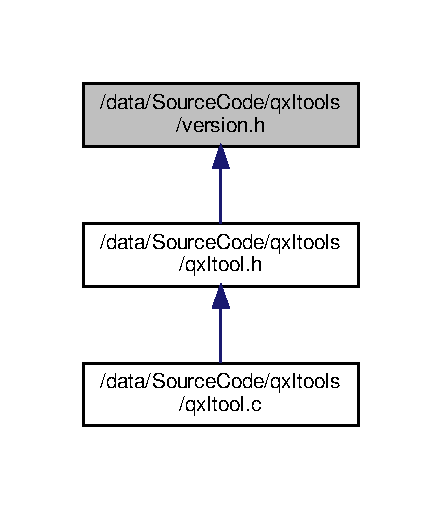
\includegraphics[width=212pt]{version_8h__dep__incl}
\end{center}
\end{figure}
\subsection*{Macros}
\begin{DoxyCompactItemize}
\item 
\#define \hyperlink{version_8h_a1c6d5de492ac61ad29aec7aa9a436bbf}{V\+E\+R\+S\+I\+ON}~\char`\"{}2.\+00\char`\"{}
\end{DoxyCompactItemize}


\subsection{Macro Definition Documentation}
\mbox{\Hypertarget{version_8h_a1c6d5de492ac61ad29aec7aa9a436bbf}\label{version_8h_a1c6d5de492ac61ad29aec7aa9a436bbf}} 
\index{version.\+h@{version.\+h}!V\+E\+R\+S\+I\+ON@{V\+E\+R\+S\+I\+ON}}
\index{V\+E\+R\+S\+I\+ON@{V\+E\+R\+S\+I\+ON}!version.\+h@{version.\+h}}
\subsubsection{\texorpdfstring{V\+E\+R\+S\+I\+ON}{VERSION}}
{\footnotesize\ttfamily \#define V\+E\+R\+S\+I\+ON~\char`\"{}2.\+00\char`\"{}}



Definition at line 1 of file version.\+h.


%--- End generated contents ---

% Index
\backmatter
\newpage
\phantomsection
\clearemptydoublepage
\addcontentsline{toc}{chapter}{Index}
\printindex

\end{document}
